%   DOCUMENT CLASS  %%%%%%%%%%%%%%%%%%%%%%%%%%%%%%%%%%%%%%%%%%%%%%%%%%%%%%%%%%%
%
%   Use the `sfuthesis` class to format your thesis. If your program does not
%   require a thesis defence, use the class option `undefended` like so:
%
%     \documentclass[undefended]{sfuthesis}
%
%   To generate a signature page for your defence, use the `sfuapproval` class
%   instead, by replacing the below line with
%
%     \documentclass{sfuapproval}
%
%   For more information about thesis formatting requirements, go to
%
%     http://www.lib.sfu.ca/help/publish/thesis
%
%   or ask a thesis advisor at the SFU Research Commons.
%

\documentclass{sfuthesis}



%   DOCUMENT METADATA  %%%%%%%%%%%%%%%%%%%%%%%%%%%%%%%%%%%%%%%%%%%%%%%%%%%%%%%%
%
%   Fill in the following information for the title page and approval page.
%

\title{Simultaneous Neural Machine Translation}
\thesistype{Depth Report}
\author{Ashkan Alinejad}
\previousdegrees{%
	M.Sc., University of Tehran, 2016\\
	B.Sc., Shahid Beheshti University, 2014}
\degree{Doctor of Philosophy}
\discipline{Computer Science}
\department{Department of Computer Science}
\faculty{}
\copyrightyear{2018}
\semester{Spring 2018}
\date{January 10, 2018}

\keywords{Neural Machine Translation; Real-Time Speech Translation; Simultaneous Translation}

\committee{%
	\chair{Pamela Isely}{Professor}
	\member{Emmett Brown}{Senior Supervisor\\Professor}
	\member{Bonnibel Bubblegum}{Supervisor\\Associate Professor}
	\member{James Moriarty}{Supervisor\\Adjunct Professor}
	\member{Kaylee Frye}{Internal Examiner\\Assistant Professor\\School of Engineering Science}
	\member{Hubert J.\ Farnsworth}{External Examiner\\Professor\\Department of Quantum Fields\\Mars University}
}



%   PACKAGES %%%%%%%%%%%%%%%%%%%%%%%%%%%%%%%%%%%%%%%%%%%%%%%%%%%%%%%%%%%%%%%%%%
%
%   Add any packages you need for your thesis here.
%   You don't need to call the following packages, which are already called in
%   the sfuthesis class file:
%
%   - appendix
%   - etoolbox
%   - fontenc
%   - geometry
%   - lmodern
%   - nowidow
%   - setspace
%   - tocloft
%
%   If you call one of the above packages (or one of their dependencies) with
%   options, you may get a "Option clash" LaTeX error. If you get this error,
%   you can fix it by removing your copy of \usepackage and passing the options
%   you need by adding
%
%       \PassOptionsToPackage{<options>}{<package>}
%
%   before \documentclass{sfuthesis}.
%
%   The following packages are a few suggestions you might find useful.
%
%   (1) amsmath and amssymb are essential if you have math in your thesis;
%       they provide useful commands like ``blackboard bold'' symbols and
%       environments for aligning equations.
%   (2) amsthm includes allows you to easily change the style and numbering of
%       theorems. It also provides an environment for proofs.
%   (3) graphicx allows you to add images with \includegraphics{filename}.
%   (4) hyperref turns your citations and cross-references into clickable
%       links, and adds metadata to the compiled PDF.
%   (5) pdfpages lets you import pages of external PDFs using the command
%       \includepdf{filename}. You will need to do this if your research
%       requires an Ethics Statement.
%
\usepackage{makecell}
\usepackage{multirow}
\usepackage{array}
\def\Tab#1{\tabular[t]{>{\rule[-1ex]{0pt}{3ex}}c}#1\endtabular}
\newcolumntype{C}{@{}c@{}}

\usepackage{amsmath}                            % (1)
\usepackage{amssymb}                            % (1)
\usepackage{amsthm}                             % (2)
\usepackage{graphicx}                           % (3)
\usepackage{caption}
\usepackage{pgfplots}
\usepackage[Algo.]{algorithm}
\usepackage[noend]{algorithmic}
\usepackage[pdfborder={0 0 0}]{hyperref}        % (4)
% \usepackage{pdfpages}                         % (5)
% ...
% ...
% ...
% ... add your own packages here!

\usepackage{tikz}
\usepackage{xcolor}
\usepackage{pifont}
\usepackage{titling}
\usetikzlibrary{plotmarks}
\DeclareRobustCommand\marksymbol[2]{\tikz[#2,scale=1.2]\pgfuseplotmark{#1};}



%   OTHER CUSTOMIZATIONS %%%%%%%%%%%%%%%%%%%%%%%%%%%%%%%%%%%%%%%%%%%%%%%%%%%%%%
%
%   Add any packages you need for your thesis here. We've started you off with
%   a few suggestions.
%
%   (1) Use a single word space between sentences. If you disable this, you
%       will have to manually control spacing around abbreviations.
%   (2) Correct the capitalization of "Chapter" and "Section" if you use the
%       \autoref macro from the `hyperref` package.
%   (3) The LaTeX thesis template defaults to one-and-a-half line spacing. If
%       your supervisor prefers double-spacing, you can redefine the
%       \defaultspacing command.
%

\frenchspacing                                    % (1)
\renewcommand*{\chapterautorefname}{Chapter}      % (2)
\renewcommand*{\sectionautorefname}{Section}      % (2)
\renewcommand*{\subsectionautorefname}{Section}   % (2)
% \renewcommand{\defaultspacing}{\doublespacing}  % (3)
% ...
% ...
% ...
% ... add your own customizations here!


\setlength\abovecaptionskip{-10pt}

%   FRONTMATTER  %%%%%%%%%%%%%%%%%%%%%%%%%%%%%%%%%%%%%%%%%%%%%%%%%%%%%%%%%%%%%%
%
%   Title page, committee page, copyright declaration, abstract,
%   dedication, acknowledgements, table of contents, etc.
%
%   If your research requires an Ethics Statement, download one from the
%   SFU library website and uncomment the appropriate lines below.
%

\begin{document}

\frontmatter
%\makecommittee{}

%\addtoToC{Ethics Statement}%
%\includepdf[pagecommand={\thispagestyle{plain}}]{ethicsstatement.pdf}%
%\clearpage
\pagebreak
\begin{titlingpage}
\hspace{0pt}
\vfill
\begin{center}
{\Large\bf Simultaneous Neural Machine Translation} \\
{\large Depth Report}\\
{\large Ashkan Alinejad}\\
{January 10, 2018}
\end{center}
\vfill
\hspace{0pt}
\end{titlingpage}
\pagebreak


\begin{abstract}
	Simultaneous machine translation removes a central assumption made by machine translation systems which is that the translation in the target language is produced only after the input source language utterance or sentence is fully received. This type of translation is particularly suited for speech to speech translation (also called conference interpretation) where waiting for the end of the sentence creates a long delay and creates an unnatural interaction between the speaker and the hearer. Most contemporary speech to speech translation systems (such as Skype Translator) use pauses in the speaker output to produce the output translation. However, a fully trainable simultaneous translation system can be more adaptive, have less latency and produce more fluent translations. There are many challenges in building a simultaneous translation model: divergent syntax of different languages, knowing when to wait and when to translate is tricky, and sometimes the translation system might need to predict what the speaker might say, or paraphrase what the speaker has said already. Neural machine translation has made great strides and has effectively replaced statistical machine translation as the state of the art. This report focuses on how neural machine translation can be modified to deal with simultaneous translation.
\end{abstract}


%\begin{dedication}
%	This is an optional page.
%\end{dedication}


%\begin{acknowledgements}
%	This is an optional page.
%\end{acknowledgements}

\addtoToC{Table of Contents}%
\tableofcontents%
\clearpage

\addtoToC{List of Tables}%
\listoftables%
\clearpage

\addtoToC{List of Figures}%
\listoffigures%
\clearpage





%   MAIN MATTER  %%%%%%%%%%%%%%%%%%%%%%%%%%%%%%%%%%%%%%%%%%%%%%%%%%%%%%%%%%%%%%
%
%   Start writing your thesis --- or start \include ing chapters --- here.
%

\mainmatter%

%++++++++++++++++++++++++++++++++++++++++++++++++++++++++++++++++++++++++++
\chapter{Introduction}
Traditionally, most machine translation research has focused on the problem of translating entire sentences at once. The translator has access to the whole sequence and there is no limit to time to be spent on analysis. The task of simultaneous translation is to translate content in real-time as it is produced, without waiting for the source sentence to be received completely. The translator must, incrementally, understand what is being said in a source language, translate it in real time into the target language, and do so in a way that maximizes fluency when there is missing information. This is a much more difficult problem. As illustrated in Figure \ref{fig:SMTVSMT}, The regular translator (right) will read from the source language (the blue arrows) until the end of the sentence and the translation process (the red arrows) starts afterwards; However, the simultaneous translator on the left side won't wait for the whole sentence and starts translating when it ensures that the translation quality is good enough.


\begin{figure}[b]
\centering
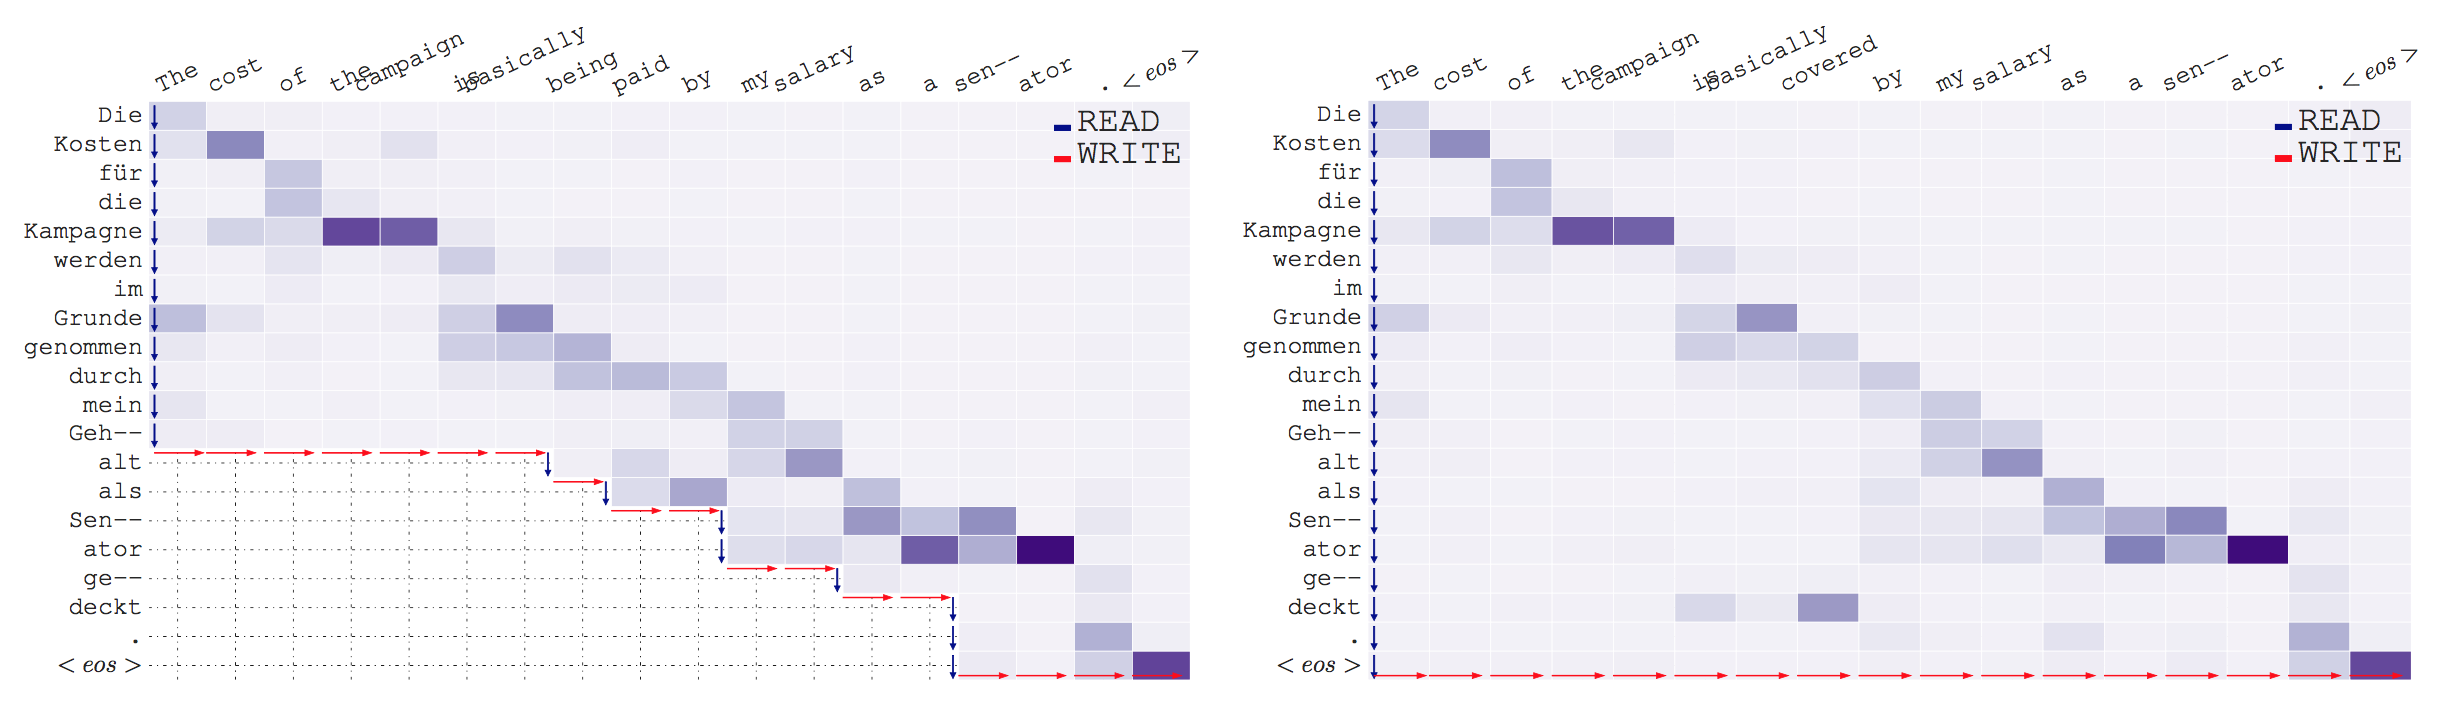
\includegraphics[scale=0.35]{./images/SMTVSMT}
\vspace{5mm}
\caption[Simultaneous MT vs Standard MT]{Simultaneous Machine Translation (left) vs Standard Machine Translation (right) systems.}
\label{fig:SMTVSMT}
\end{figure}

In this report we will first briefly describe RNN models and evaluation metrics for simultaneous machine translation (SMT). We will go through some of the previous approaches toward solving SMT problem (section \ref{chap:TS}), and then the standard NMT framework with attention mechanism will be explained afterwards in Chapter \ref{chap:NMT}. Various successful methods for applying Neural Networks in SMT is explained in Chapter \ref{chap:SNMT}. Finally, we will compare empirical evaluation of SNMT systems in Chapter \ref{chap:results}.
\section{Recurrent Neural Networks} \label{sec:RNN}

Recurrent Neural Networks (RNNs) are feedforward networks augmented by the inclusion of edges that span adjacent time steps, introducing a notion of time to the model \cite{zachary:2015:arxive}. The standard RNN is a nonlinear neural network that maps sequences to sequences. The most important aspect of having recurrent edges is that input at time $t$, not only influence the output at time $t$, but it can also affect results at future time steps. Hence it can capture the dynamics of arbitrary sequences without changing its structure.

Given an input sequence $\text{X} = \{ x_1, \dots, x_n \}$, the RNN computes the sequence of hidden states $\text{H} = \{ h_1, \dots, h_n \}$ and the sequence of outputs $\text{Y} = \{ y_1, \dots, y_n \}$ using the following two equations:
\begin{align*}
\centering
h_t &= \sigma (W_{hx} x_t + W_{hh} h_{t-1} + b_h)\\
y_t &= \delta (W_{hy} h_t + b_y)
\end{align*}
Where $W$ and $b$ are weights and biases of the network and should be updated during training. $\sigma$ and $\delta$ are nonlinear functions for the hidden and output layers respectively. Figure \ref{fig:RNN0} illustrates structure of a simple RNN for different time steps.

\begin{figure}[t]
\centering
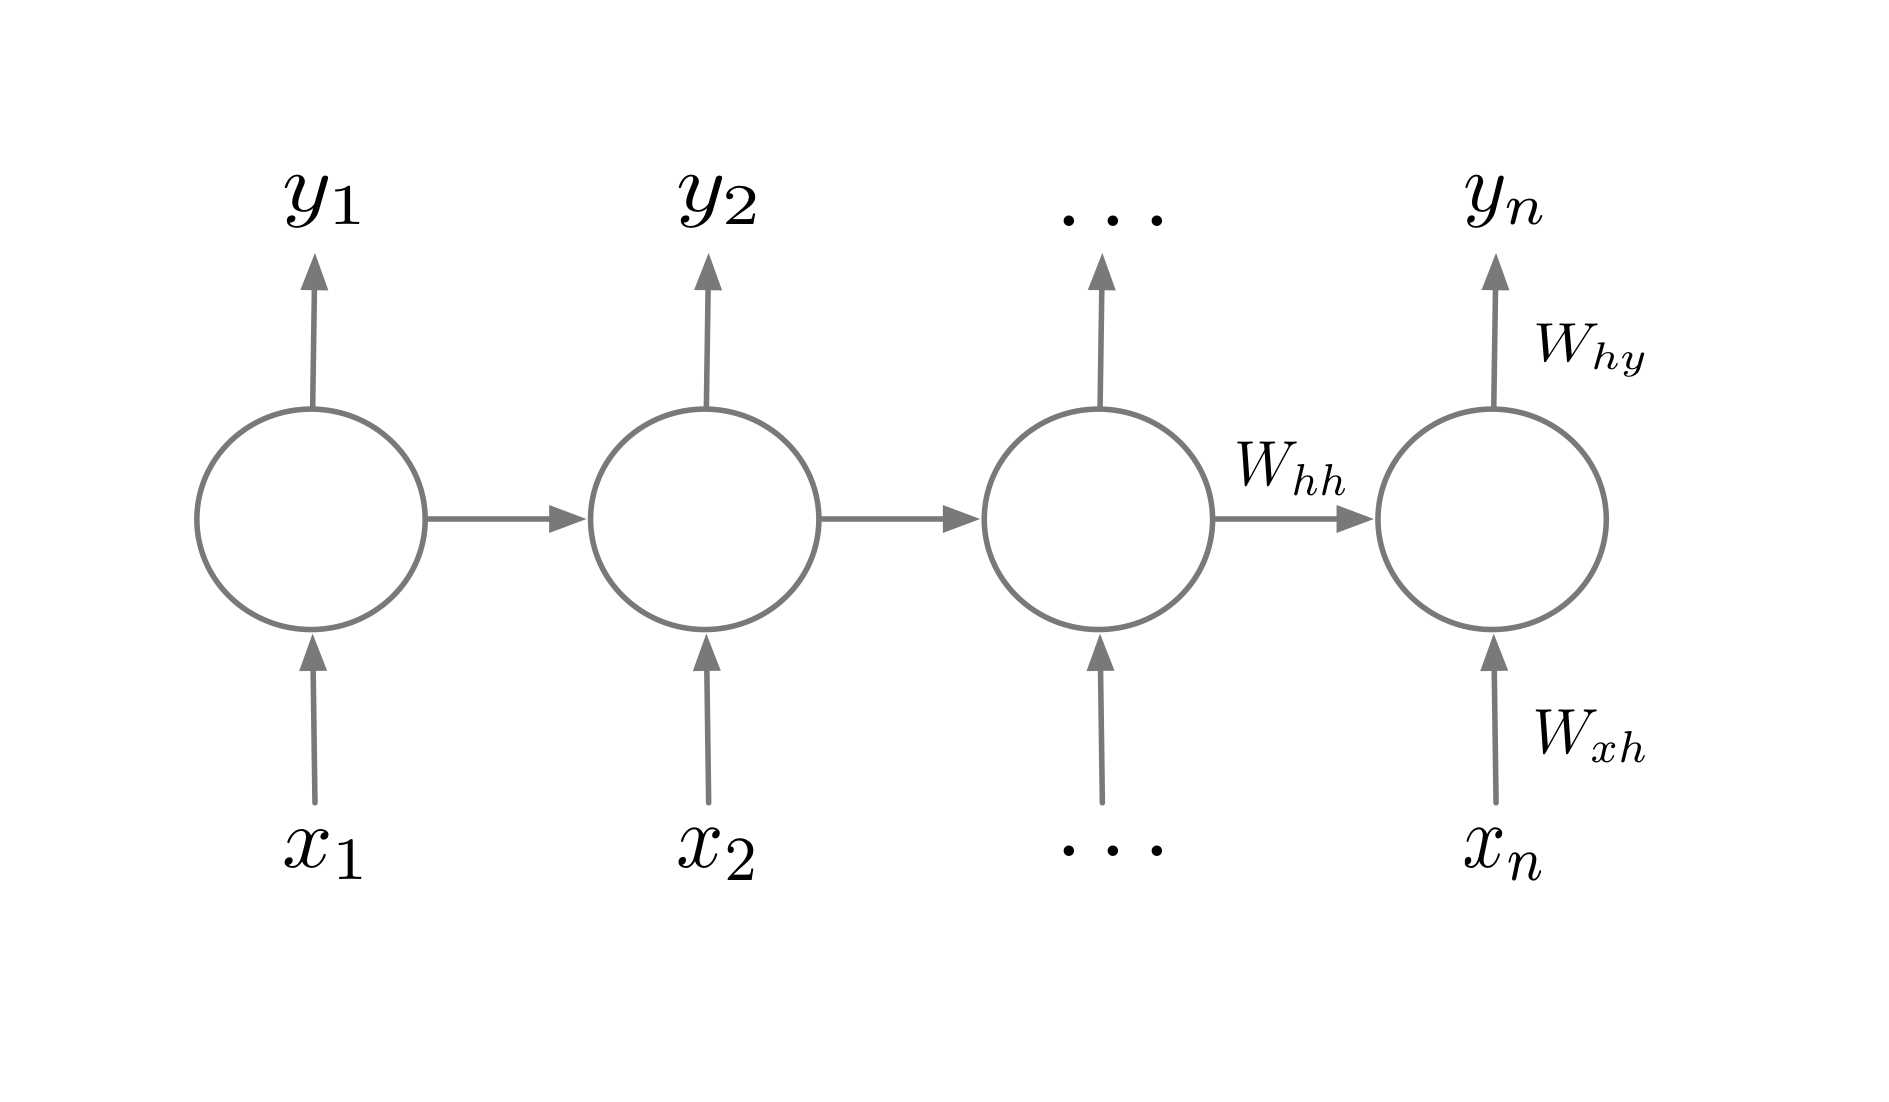
\includegraphics[scale=0.15]{./images/RNN}
\caption[Recurrent Neural Network]{Recurrent Neural Network. Weights $W_{xh}$, $W_{hh}$ and $W_{hy}$ are shared between different time steps}
\label{fig:RNN0}
\end{figure}

While the derivation of parameters of the RNNs can be computed using Back Propagation Through Time (BPTT) algorithm \cite{werbos:1990:IEEE}, learning with recurrent networks has long been considered difficult; Especially for problems with long-term dependencies \cite{Bengio:1994:LLD}, since the networks couldn't keep information for many time steps. In addition, when the sequences are long and we need to back propagate through many time steps, the problem of \textit{vanishing} or \textit{exploding} gradients may occur, which make it even harder to stabilize the network during training. Exploding gradients refer to the problem of increasing gradients exponentially as we back propagate through many time steps which may lead the training process unstable. Vanishing gradients, on the other hand, is the problem of decreasing gradients rapidly, which makes back propagation unsuccessful in capturing long-term dependencies of sequences \cite{Bengio:1994:LLD, Hochreiter:1997:LSM, martens:2011:ICML}.

After proposing Long Short-Term Memory (LSTM) networks by Hochreiter and Schmidhuber \cite{Hochreiter:1997:LSM} as solution to the vanishing and exploding gradients, and Bidirectional Recurrent Neural Networks (BRNN) by Schuster and Paliwal \cite{Schuster:1997:BRNN} in order to improve the results of the RNNs, the recurrent architectures become more successful. The main idea of LSTM networks is to replace basic standard nodes in network with more complex memory-included cells that can carry more information to the future time steps. We will discuss more about them in \ref{sub:LSTM}. The idea behind BRNNs and how they can improve results will be discussed in Chapter \ref{chap:NMT}.

\subsection{Long Short-Term Memory} \label{sub:LSTM}
Long Short-Term Memory Networks serves as an underlying computational building blocks of most modern NMT systems. The structure of the network looks like standard recurrent neural network with one hidden layer; However each node in hidden layer is replaced by \textit{memory cell} as in Figure \ref{fig:LSTM0}.

\begin{figure}[t]
\centering
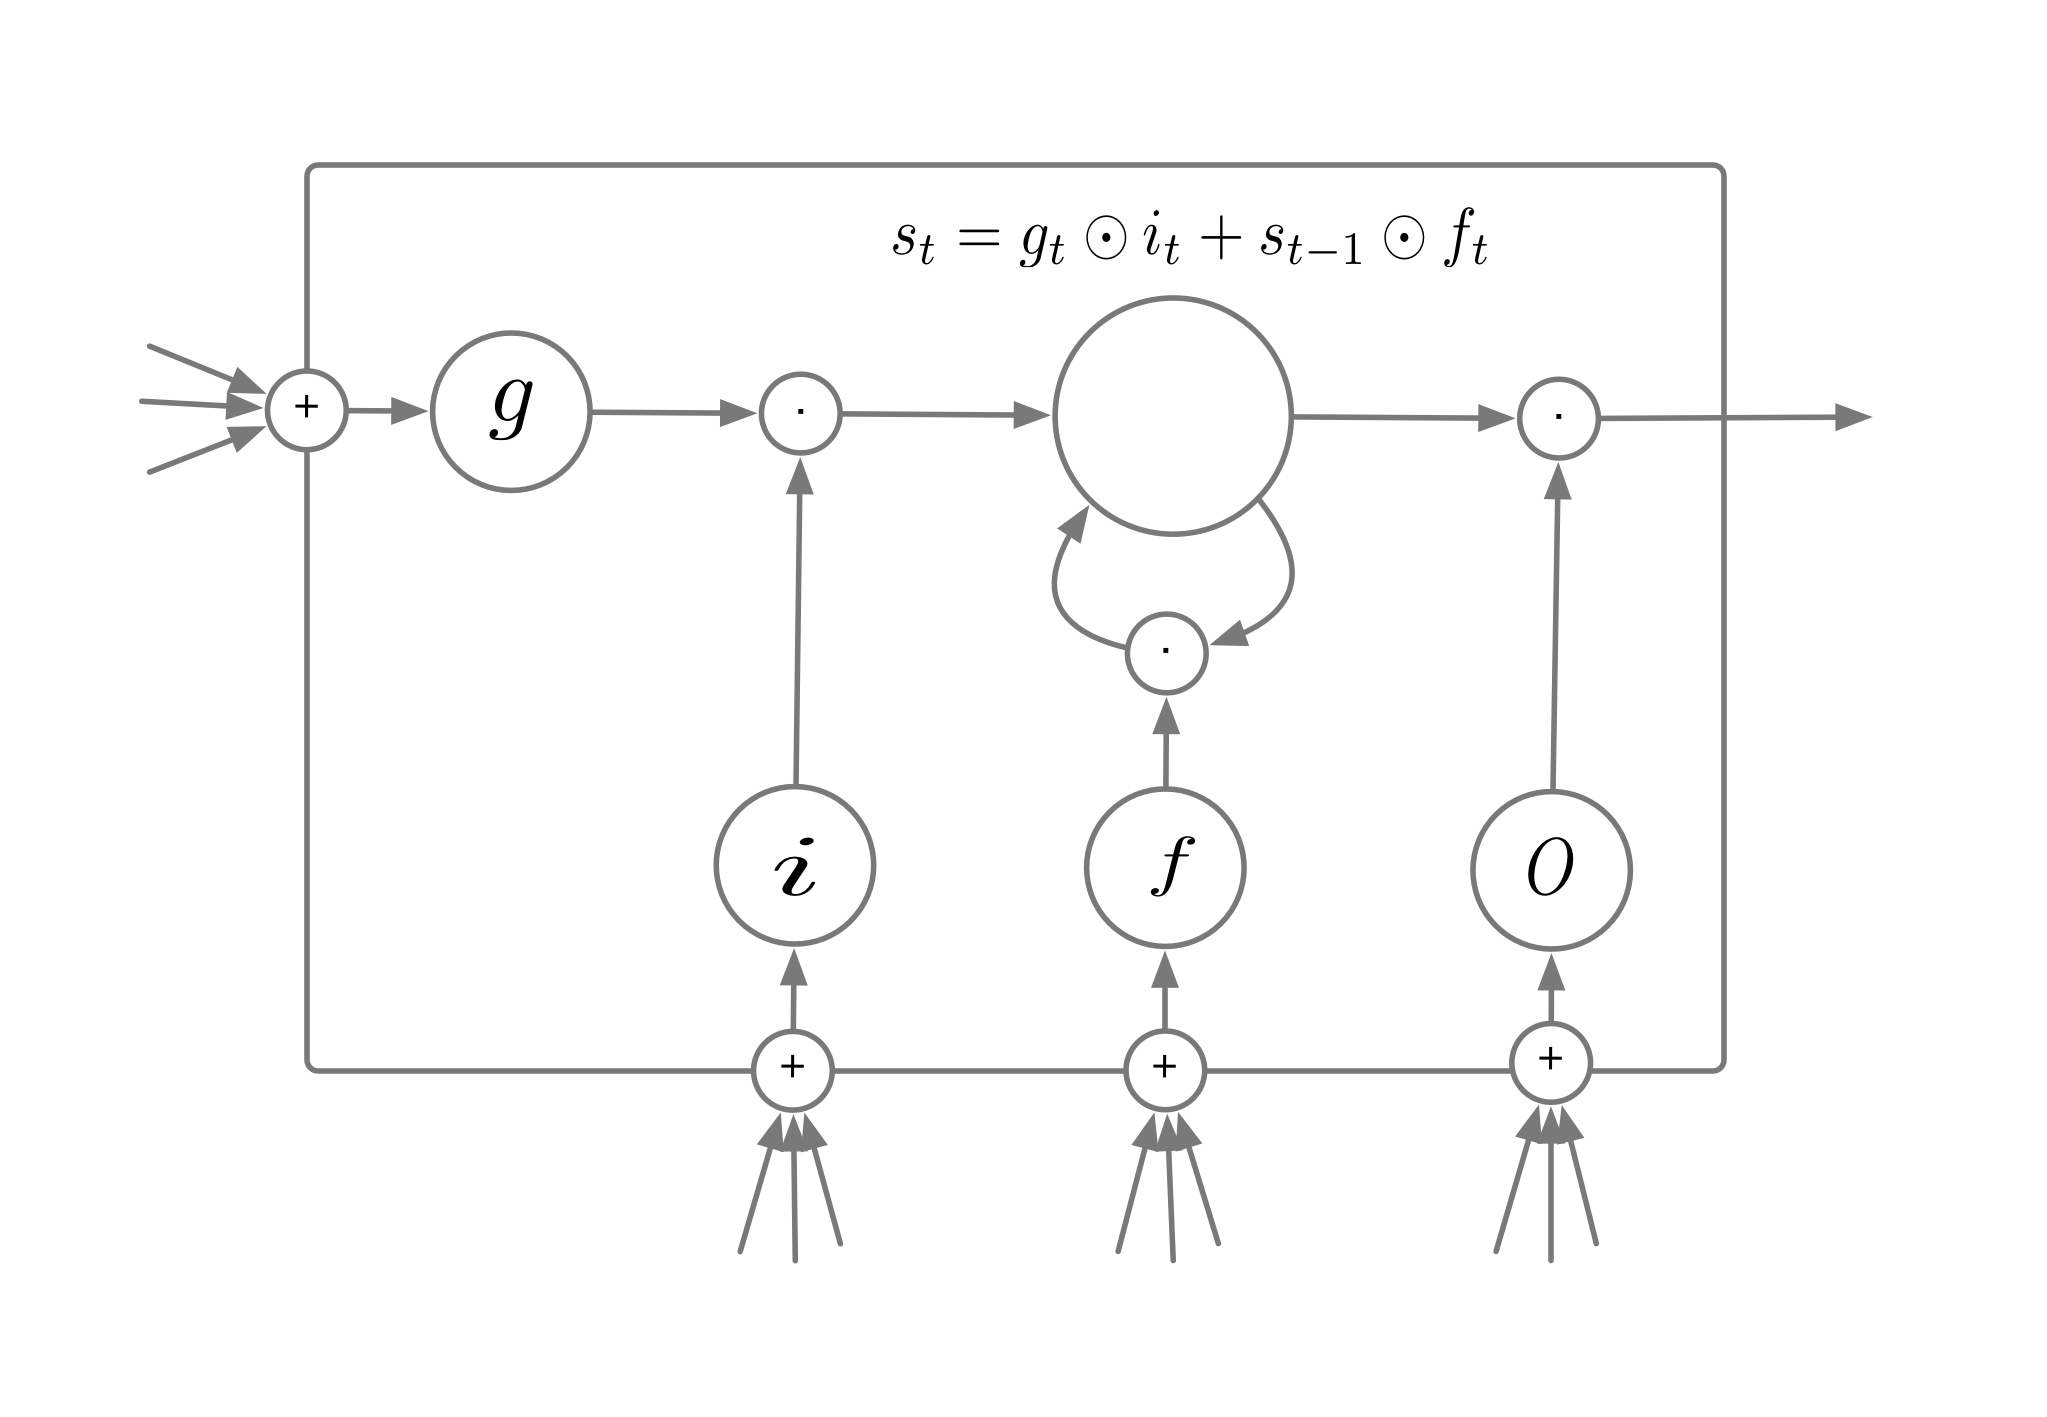
\includegraphics[scale=0.15]{./images/LSTM}
\caption[LSTM memory cell]{A LSTM memory cell as described by Gers et al. \cite{Gers:2000:LFC}}
\label{fig:LSTM0}
\end{figure}

A memory cell consists of a linear unit called "internal state" and a number of simpler nodes which serve as \textit{gating} units, in order to control data flow in each cell, easier. They are "\textit{gate}" since when their value is zero, the data wont be allowed to enter to the cell. Internal state is a linear unit with a self-connected edge with weight 1, which allows gradients to stay in cell for indefinite amount of time without vanishing or exploding. In the original LSTM paper proposed by Hochreiter et al. \cite{Hochreiter:1997:LSM} there is no forget gate; However, Gers et al. \cite{Gers:2000:LFC} show that learning to flush the information kept in internal state can improve results.

Mathematically speaking, all the calculations in an LSTM memory cell with forget gates can be described by the following equations:
\begin{align}
\centering
&g_t = \phi (W_{gx}x_t + W_{gh}h_{t-1} + b_g) \label{eq:1.1}\\
&i_t = \sigma (W_{ix}x_t + W_{ih}h_{t-1} + b_i) \label{eq:1.2}\\
&f_t = \sigma (W_{fx}x_t + W_{fh}h_{t-1} + b_f) \label{eq:1.3}\\
&o_t = \sigma (W_{ox}x_t + W_{oh}h_{t-1} + b_o) \label{eq:1.4}\\ 
&s_t = g_t \odot i_i + s_{t-1} \odot f_t \label{eq:1.5}\\
&h_t = \phi(s_t) \odot o_t
\end{align}
The product $\odot$ denotes element-wise multiplication. Equations \ref{eq:1.2}, \ref{eq:1.3} and \ref{eq:1.4} describe input gate, forget gate and output gate respectively. The basic LSTM network without forget gate can be obtained be setting $f_t = 1$. In addition, if we set all input gates to 1, all forget gates to zero, and all output gates to 1, then we will get almost a simple standard RNN. 

\subsection{Gated Recurrent Units}

The idea behind Gated Recurrent Units (GRU) which was proposed by Cho et al. \cite{cho:2014:arxive}, is very similar to LSTM memory cell, as it has the same gating mechanism. In contrast to LSTM, GRUs have fewer parameters, and there will be only two \textit{update} and \textit{reset} gates. The network can be described as:
\begin{align}
\centering
&z_t = \sigma (W_{zx}x_t + W_{zs}s_{t-1} + b_z) \label{eq:1.7}\\
&r_t = \sigma (W_{rx}x_t + W_{rs}s_{t-1} + b_r) \label{eq:1.8}\\
&h_t = \phi (W_{hx}x_t + W_{hs}(s_{t-1} \odot r_t )) \label{eq:1.9}\\ 
&s_t = (1 - z_t) \odot h_t + z_{t} \odot s_{t-1} \label{eq:1.10}
\end{align}
As we can see, there is no internal state in GRU and the second non-linearity won't be applied to the output. Although the number of parameters in GRU is less than LSTM and training is a bit faster, the empirical evaluations of Jozefowicz et al. \cite{Jozefowicz:2015:ICML} showed that adding a bias of 1 to the LSTM's forget gate closes the gap between the LSTM and the GRU.


\section{Evaluation Methods}
In standard NMT framework translation quality is primary metric for evaluating various translation systems. However, simultaneous translation requires balancing the trade-off between translation quality and time delay to ensure that users receive translated content in an expeditious manner \cite{mieno:2015:interspeech}. Consequently, in this section we will describe various evaluation metrics for both quality and delay in MT systems.
\subsection{Quality} \label{subsec:quality}
Although human evaluations for the quality of machine translation (MT) weigh many aspects of translation, including adequacy, fidelity , and fluency of the translation \cite{hovy:1999:toward}, they are expensive and time-consuming. As a result, automatic evaluation techniques such as \emph{BLEU score} \cite{Papineni:2002:ACL} has been widely used in MT systems. Here, we will discuss the most commonly used evaluation metrics for quality:\\
\begin{itemize}
    \item \textbf{ Standard BLEU}\\
    In recent years BLEU became the de facto standard machine translation (MT) evaluation metric \cite{chen:2014:ACL}. It is based on the degree of n-gram overlapping between the strings of words produced by the machine and the human translation references at the corpus level. BLEU is usually computed for n-grams of size 1 to 4 with the coefficient of brevity penalty (BP).

\begin{align*}
\centering
\text{BLEU} &= \text{BP} \times \bigg( \prod_{n=1}^{N} \frac{m_n}{l_n} \bigg)^\frac{1}{N}
\end{align*}

\begin{align*}
\centering
\text{BP} &= 
\begin{cases}
1 & \text{if} \ c>r\\
e^{1-\frac{r}{c}} & \text{if} \ c\leq r
\end{cases}
\end{align*}
Where $m_n$ is the number of matched n-grams between
translation and its reference, and $l_n$ is the total number of n-grams in the translation. $c$ is the total length of candidate translation corpus, and $r$ refers to the sum of effective reference sentence length in the corpus.

    \item \textbf{ Smooth BLEU}\\
    One of the main criticisms of BLEU is that since it computes a geometric mean of n-gram precisions, if a higher order n-gram precision (e.g. n = 4) of a sentence is 0, then the BLEU score of the entire sentence is 0, no matter how many 1-grams or 2-grams are matched. Among several smoothing techniques proposed to address this problem, the smoothing technique suggested by Lin et al. \cite{Lin:2004:ACL} is the most widely used. It adds 1 to the matched n-gram count and the total n-gram count for n ranging from 2 to $N$.
    $$m'_n = m_n + 1 \qquad \text{for}\ n\ \text{in}\ 2 \dots N$$
    $$l'_n = l_n + 1 \qquad \text{for}\ n\ \text{in}\ 2 \dots N$$
\end{itemize}
\subsection{Delay} \label{subsec:delay}
Another critical feature in real-time machine translation systems is delay which means how much time is wasted for reading when translating each word. there is no unique formulation for delay and various methods use their own definition to report rapidity of their systems. The more common and accurate choices in practice for delay function is \emph{Average Proportion} and \emph{Consecutive Wait} which we will describe them: 
\begin{itemize}
    \item \textbf{Average Proportion (AP)}\\
    Cho et al. \cite{cho:2016:Arxive} defined AP as average number of source words needed when translating each word. In other words, $d(X, Y)$ can be computed as:
    $$d(X, Y) = \frac{1}{|X||Y|} \sum_t s(t)$$
    Where $X$, $Y$ are the source and decoded sequences respectively, and $s(t)$ denote the number of source words been waited when decoding each word.
    \item \textbf{Consecutive Wait (CW)}\\
    CW as is defined by Gu et al. \cite{gu:2017:EACL} is how many words were waited for (READ) consecutively between translating two words. It is defined at each time step is equal to the length of the current segment. CW can be computed at each time step as: 
    \begin{align*}
        c_t = 
        \begin{cases}
        c_{t-1} + 1 & a_t = \text{READ}\\
        0           & a_t = \text{WRITE}
        \end{cases}
    \end{align*}
\end{itemize}
\vspace{0.2cm}
\section{Traditional Systems} \label{chap:TS} %%%%%%%%%%%%% Label should be updated
Before starting the new wave of modern neural architectures, a number of statistical methods have been proposed to address the problem of simultaneous translation, mostly in the context of speech translation \cite{Bangalore:2012:NAACL, Fugen:2007:MT}. In this section we will briefly discuss four major threads and challenges from statistical approaches. Some of these challenges remained unsolved in modern architectures.

\begin{enumerate}
    \item \textbf{Segmentation}\\
    In real-time translation, interpreter must split a constant stream of words into translatable segments, in a way that maximizes the translation quality and minimizes segment length. The statistical approaches for splitting sentences can be divided into two main groups: \emph{sentence segmentation} and \emph{incremental decoding}. In incremental decoding, incoming words are fed into the decoder one-by-one, and the decoder updates its internal state. The decoder is responsible to decide when to begin the translation process and when to output the translation. In sentence segmentation, the focus is on splitting sentences and as soon as a segment is recognized, it is given to a decoder to generate and output the translation for that segment.
    \item \textbf{Prediction}\\
    In real-time translation we do not have access to future time steps. Consequently when translating from subject-object-verb (SOV) languages like German to subject-verb-object (SVO) languages like English, since the main verb may appear later in an SOV language, for the translation to be truly incremental, the verb, copula, or other sentence-final components must be predicted and translated before they are actualized in the source sentence.\\
    Konieczny et al. \cite{doring:2003:ICCS} predict verbs with a recurrent neural network, but Matsubara et al. \cite{matsubarayx:2000:NLP} was the first to use verb predictions as part of a simultaneous interpretation system. They use pattern matching-based predictions of English verbs. In contrast, Grissom II et al. \cite{Grissom:2014:EMNLP} use a statistical approach, using n-gram models to predict German verbs and particles.
    \item \textbf{Rewording}\\
    Prediction task is inherently hard and most of the time it's inaccurate. As another solution for SOV-SVO language pair translation, one can apply syntactic transformations to make the word order of one language closer to the other. In other words, rewording is changing the standard way of wording output to prevent from long delays. He at al. \cite{he:2015:EMNLP} proposed to rewrite the reference translation in a way that uses the original lexicon, obeys standard grammar rules of the target language, preserves the original semantics. They then train the MT system with the rewritten references so that it learns how to produce low-latency translations from the data.
    \item \textbf{Evaluation}\\
    Another important question for simultaneous translation systems is that how should we evaluate our translator. It's not trivial what is the best method for rewarding the system according to its accuracy and rapidity. Mieno et al. \cite{mieno:2015:interspeech} devised an evaluation measure for simultaneous speech translation that simultaneously considers delay and accuracy and found out that considering both speed and translation accuracy in the evaluation of simultaneous speech translation systems results in more effective evaluation.
\end{enumerate}


%++++++++++++++++++++++++++++++++++++++++++++++++++++++++++++++++++++++++++
\chapter{Neural Machine Translation} \label{chap:NMT}
Neural Networks can be seen as an essential component in most of recent approaches in the field of machine translation. In section \ref{sec:RNN} we have reviewed various components of RNNs\footnote{Recurrent Neural Networks} . During this Chapter, we will describe how we can use them to build translation systems that can extract semantic information from source language and follow the syntactical structure of target language in order to produce translated words.

\section{Neural Translation Models} \label{sec:NTM}
Most of the state-of-the-art approaches toward solving Machine Translation uses the Encoder-Decoder architecture with attention; However, since adding attention mechanism makes the structure more complex, we will start with describing simple Encoder-Decoder translation systems in the next section. Later, in \ref{sub:attention} we will demonstrate how attention mechanism affects the translation process.
\subsection{Encoder-Decoder structure} \label{sub:EncDec}
The very basic neural structure that can generate reasonable translations is what is called the \textbf{Encoder-Decoder} model \cite{Chrisman:1991:EncDec, Sutskever:2014:NIPS, cho:2014:emnlp}. The concept of this model is to use stacked layers of LSTM or GRU cells in order to \emph{encode} the whole source sentence into a real-valued vector. Then we can feed this vector to our second neural network to \emph{decode} it and produce translated words one at a time. see Figure \ref{fig:EncDec0} for illustration.\\
More mathematically, our network at time step $t$ will receive a numerical representation of word $x_t$ from the source sentence $X = \{x_1, \dots, x_T\}$. Then it will combine them with output of encoder at previous time step and passes them to a non-linear function. In other words: $h_t = f(x_t, h_{t-1})$, where $f$ is a non-linear function (e.g. Tanh, Sigmoid, ...). Once the encoder receives the <eos> word, it will start to compute the final encoder's context vector $h_T$.\\
In the decoder component, we will use the predicted word from previous time step $y_{i-1}$, previous decoder output $s_{i-1}$ as well as $h_T$, as an input for decoder's neural network. We will compute $s_{i}$, similar to encoder's context vector, with $s_{i} = g(y_{i-1}, s_{i-1}, h_{T})$, where $g$ is a non-linear function. Then we will pass $s_i$ through a softmax layer in order to compute the probability $P(y_i | X, y_{<i})$.  We will choose $y_i$ that maximizes the probability. i.e. $i = \arg\max_{y_i} P(y_i | X, y_{<i}$).\\
This is the very basic, yet powerful structure of the encoder-decoder model and while there are lots of neural models for machine translation, these can be seen as extensions to this model. In \cite{Sutskever:2014:NIPS} it is shown that with some refinements (E.g. using BiLSTM instead of LSTM as encoder), the encoder-decoder structure can beat most of the approaches with many years of research in their background. We will talk about these techniques in the next two sections.
\begin{figure}[t]
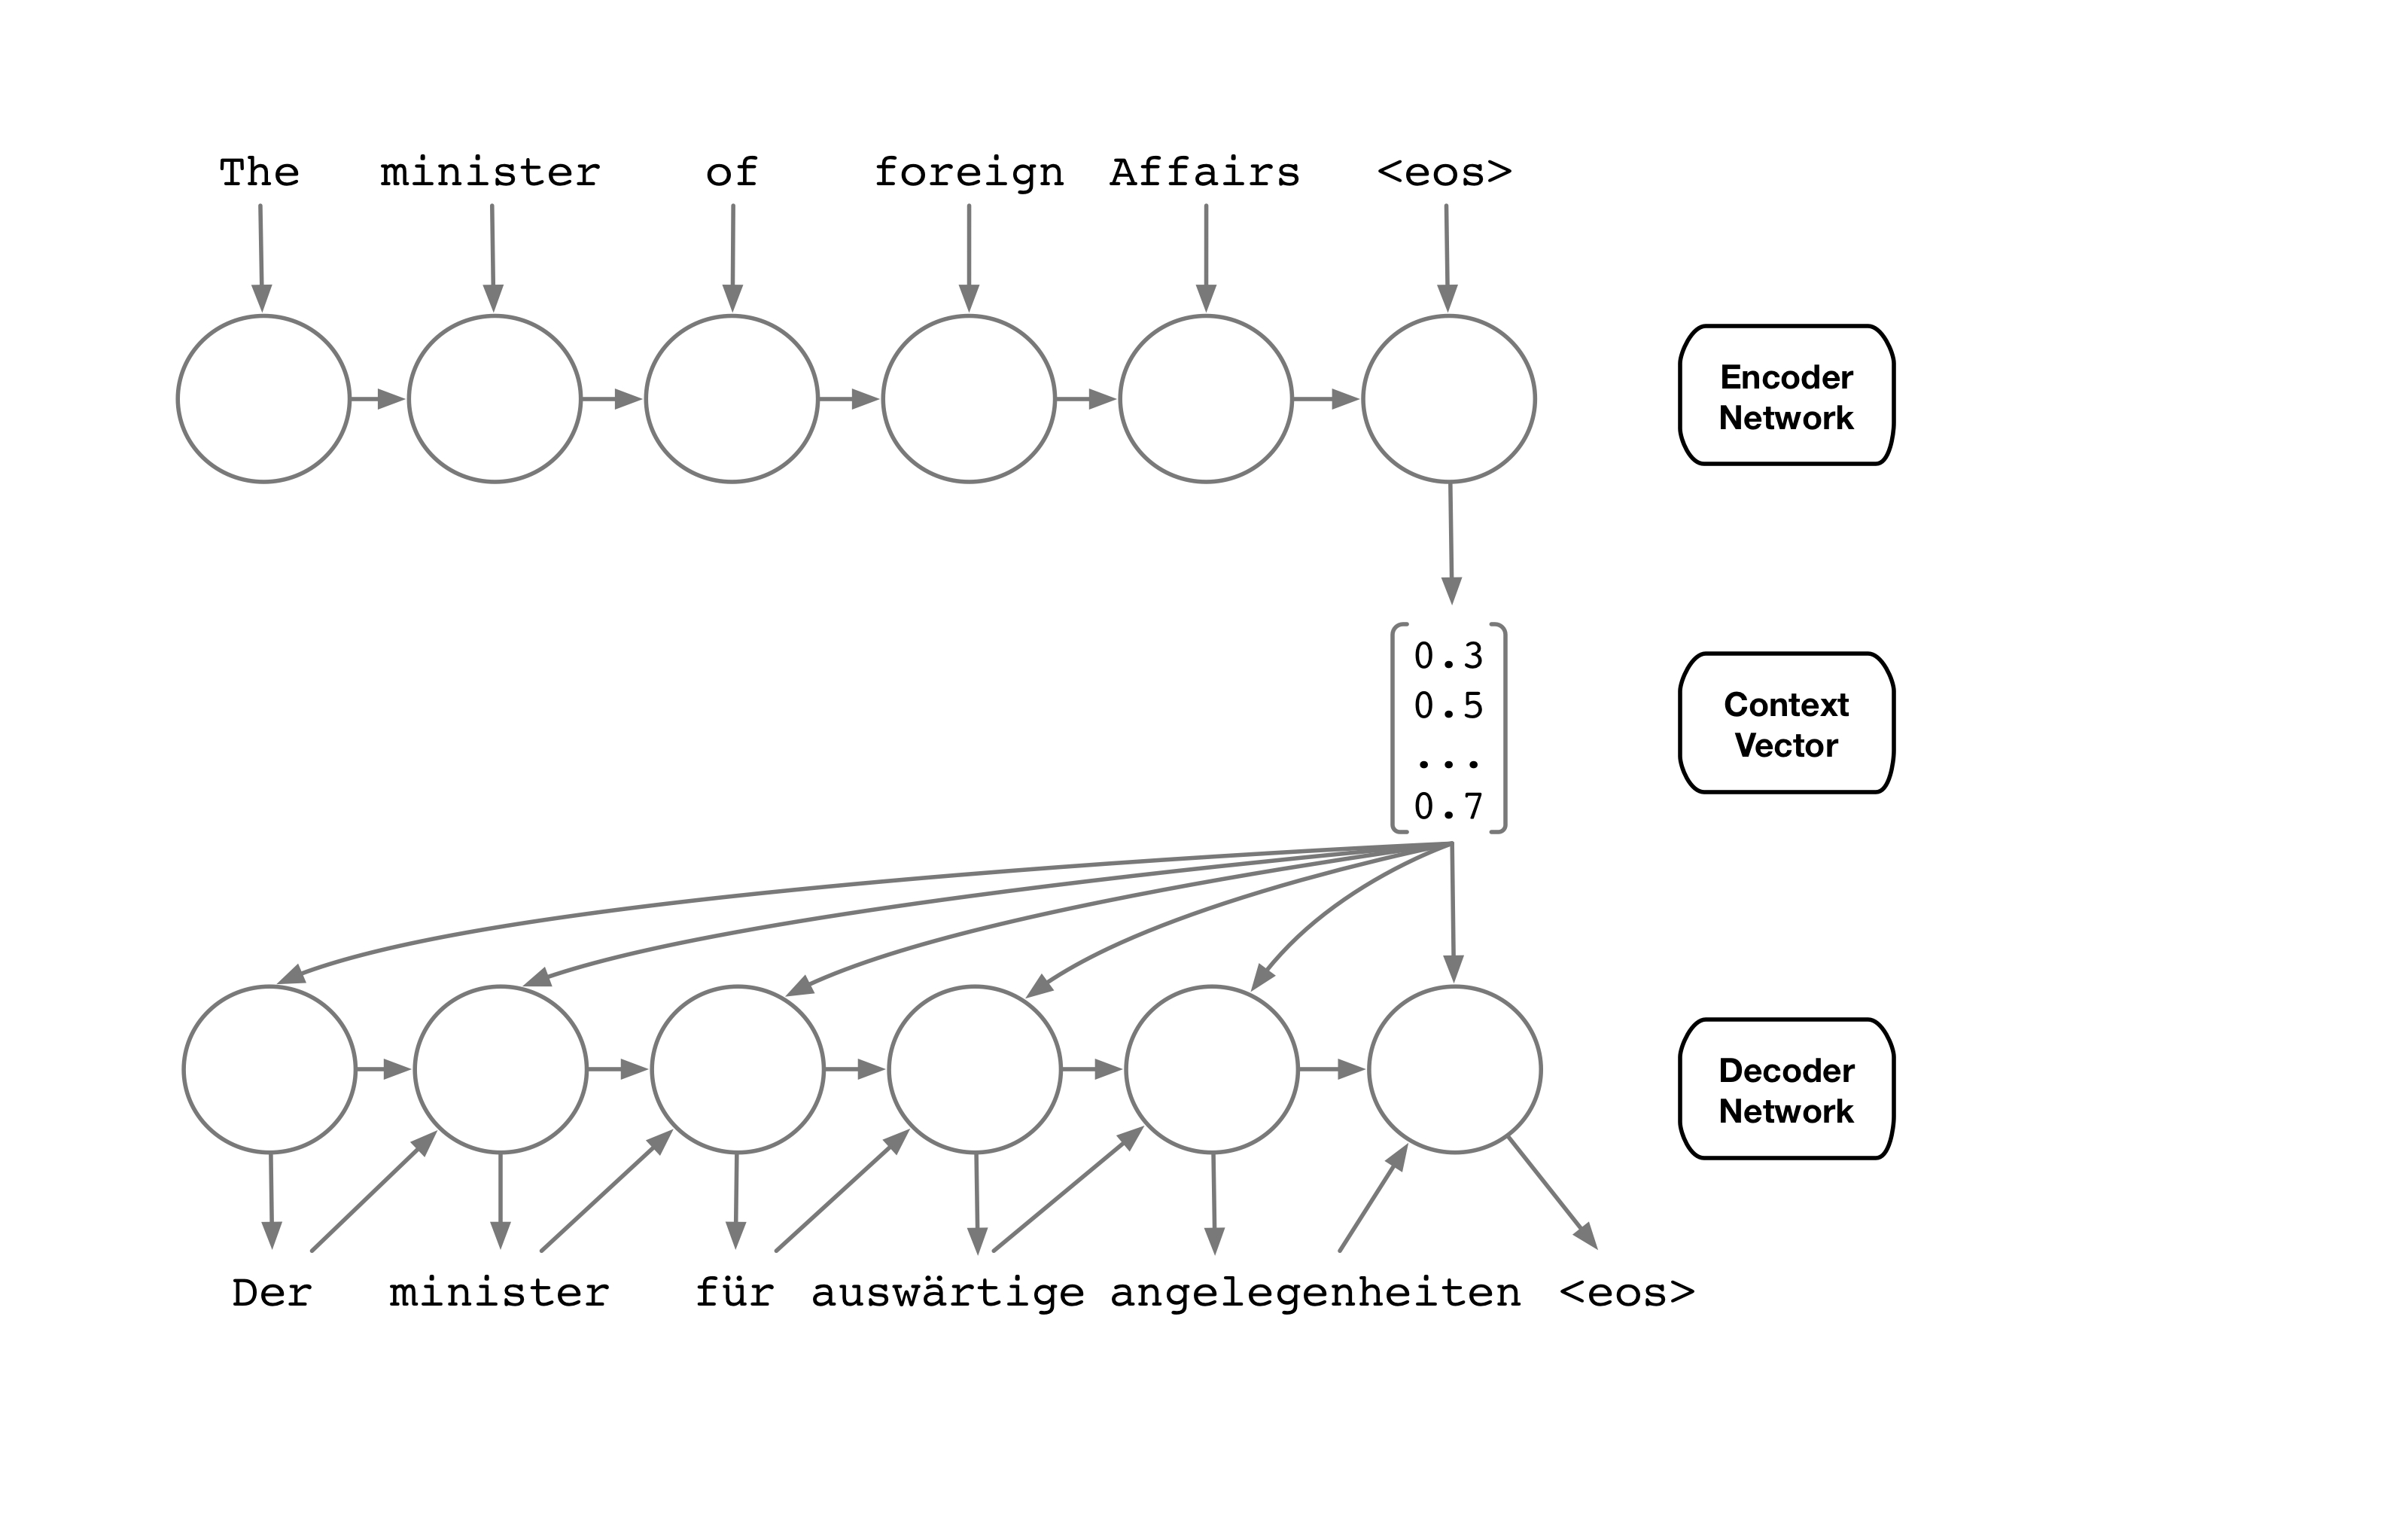
\includegraphics[scale=0.15]{./images/EncDec0}
\caption{Structure of an Encoder-Decoder model.}
\label{fig:EncDec0}
\end{figure}

\subsection{Bidirectional RNNs}
Bidirectional RNNs (BRNN) \cite{Schuster:1997:BRNN} extend the unidirectional RNN by introducing a second hidden layer with connections that flow in opposite temporal view. The first hidden layer passes the activations forward, which connects the previous time steps to the current time step; While the second layer have connections in opposite direction so that the information from future can be observed by current time step. The nodes in both hidden layers are connected to the nodes to previous and next layers. The computations in a BRNN layer can be described by three equations:
\begin{align*}
    h_t &= \sigma (W_{hx} x_t + W_{hh} h_{t-1} + b_h)\\
    z_t &= \sigma (W_{zx} x_t + W_{zz} z_{t+1} + b_z)\\
    y_t &= \delta (W_{yh} h_t + W_{yz} z_t + b_y)
\end{align*}
One limitation of BRNN is that it cannot be applied to online or real-time applications, since it's not possible to receive information from future. But in batch procedures having access to the whole sequence is reasonable assumption and BRNNs can improve results.
\subsection{Attention Mechanism} \label{sub:attention}
We are only one step away to look at the state-of-the-art translation model which is the encoder-decoder model with attention mechanism. As we have seen in \ref{sub:EncDec}, the encoder-decoder networks forces the encoder to keep all the information required for decoding into a fixed-dimensional context vector. On the other side of this structure, the decoder only have access to this context vector and it is supposed to produce the whole translation using this fixed representation of input.\\
With keeping these restrictions in mind, although the architecture works well, as the length of sentences grows, the decoder's performance decreases a lot. In order to fix these constraints, Bahdanau et al. \cite{Bahdanau:2014:Attention} proposes the attention mechanism. The main idea is that instead of using the last state of the encoder's context vector, the decoder is able to use a weighted combination of encoder's output at different time steps. As a result, Not only the decoder would be powerful, but it would also be much more easier for encoder to encode input sentences at each time step. \\
More concretely, the first component of this structure encodes the embeddings of input words $X=\{ x_1, \dots, x_{T_s} \}$ into context vectors $H = \{ h_1, \dots, h_{T_s} \}$. It can be done by utilizing a bidirectional RNN:

$$h_i = \phi_{\text{BiRNN}}(h_{i-1}, x_i)$$
On decoder side we will have:
\begin{align}
\centering
&\alpha_i^\tau = \phi_{\text{ATTN}}(z_{\tau -1}, h_i)  \label{eq:att1}
\end{align}
\begin{align}
\centering
&c_\tau = \sum_{i=1}^{T_x} \alpha_i^\tau h_i  \label{eq:att2}
\end{align}
\begin{align}
\centering
&z_\tau = \phi_{\text{DEC}}(z_{\tau -1}, y_{\tau -1}, c_\tau)  \label{eq:att3}
\end{align}
\begin{align}
\centering
&p(y|y_{<\tau}, H) \propto \text{exp} [\phi_{out} (z_{\tau}) ]  \label{eq:att4}
\end{align}
\begin{align}
\centering
&y_{\tau} = \arg \max_y p(y|y_{<\tau}, H)
\end{align}
In equation \ref{eq:att1}, $z_{\tau - 1}$ is the decoder's context vector at previous time step and $\phi_{\text{ATTN}}$ is the attention function which can be any function that measures how well the input at position $i$ is related to output at time step $\tau$. The most commonly used function is the original formula presented by Bahdanau et al \cite{Bahdanau:2014:Attention} which employs a multi-layer feedforward neural network. We then pass these scores to a softmax function in order to make their summation equal to one. The output of attention layer in equation \ref{eq:att2} is using $\alpha_i^\tau$ as probability for computing a weighted average over the encoder's context vector.


\begin{figure}[t]
\centering
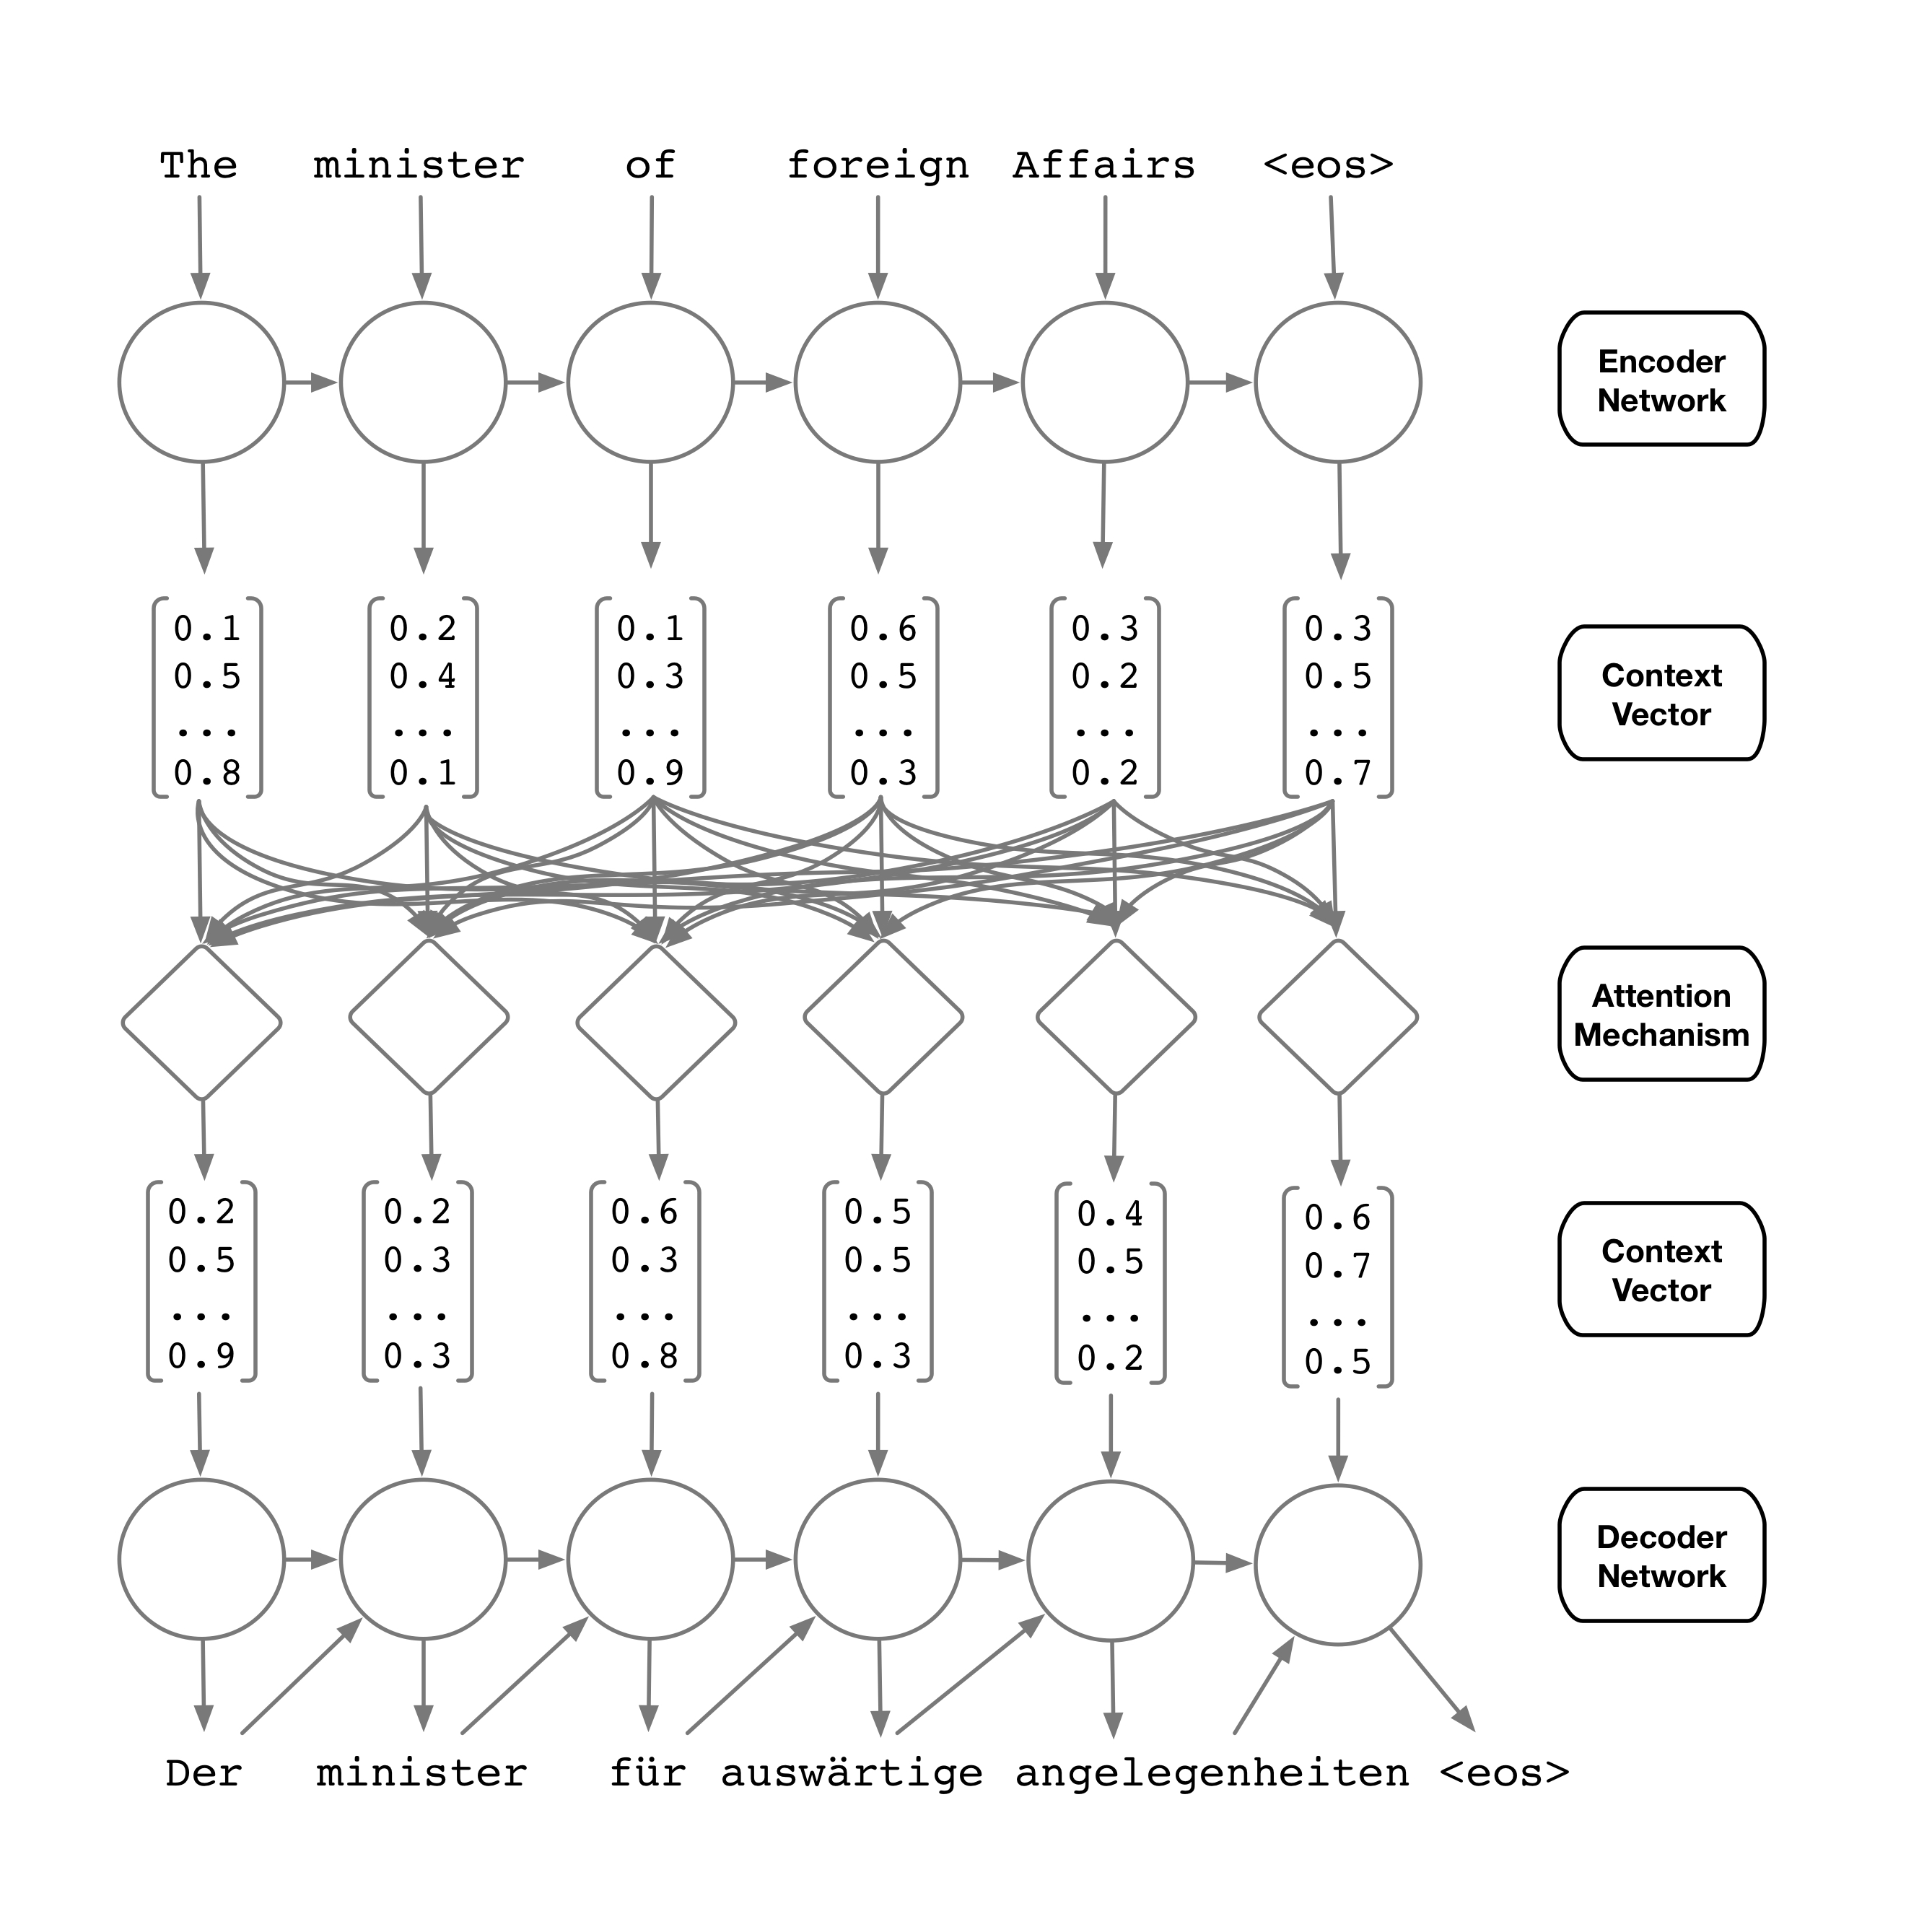
\includegraphics[scale=0.15]{./images/attention}
\caption{Structure of an Encoder-Decoder model with Attention mechanism.}
\label{fig:EncDec0}
\end{figure}


%++++++++++++++++++++++++++++++++++++++++++++++++++++++++++++++++++++++++++
\chapter{Real-Time Neural Machine Translation} \label{chap:SNMT}
In this Chapter, we will describe the framework for applying neural networks in simultaneous machine translation.\\
The most successful simultaneous neural frameworks for machine translation stem from two main papers in 2016. The first paper by Cho et al. \cite{cho:2016:Arxive} introduce a separate agent with a fixed heuristic policy for segmentation; And the second paper by Satija et al. \cite{harsh:2016:ICML} proposed the first trainable agent to decide when to start translating. Both models can be divided into two primary components which is illustrated in Figure \ref{fig:SNMT0}. The first part is Environment which receives the input words $X=\{x_1, \dots, x_{T_x}\}$ from the source language and incrementally generates translated words $W = \{ w_1, \dots, w_{T_w} \}$ in the target language. we will explain it in more details in section \ref{sec:NTE}. the other component is Agent which consecutively decides at each time $t$ whether to READ or WRITE and then controls the Environment. Hence the number of Agent's decisions $T$ can be written as $T = T_x + T_w$. A number of state-of-the-art strategies for the Agent will be discussed in section \ref{sec:Agent}. Note that since the agent selects only some the outputs of the translation environment as actual output of the system, we will use $y_t$ as the candidate output at time $t$, and $w_i$ as the actual output.

\begin{figure}[h]
\centering
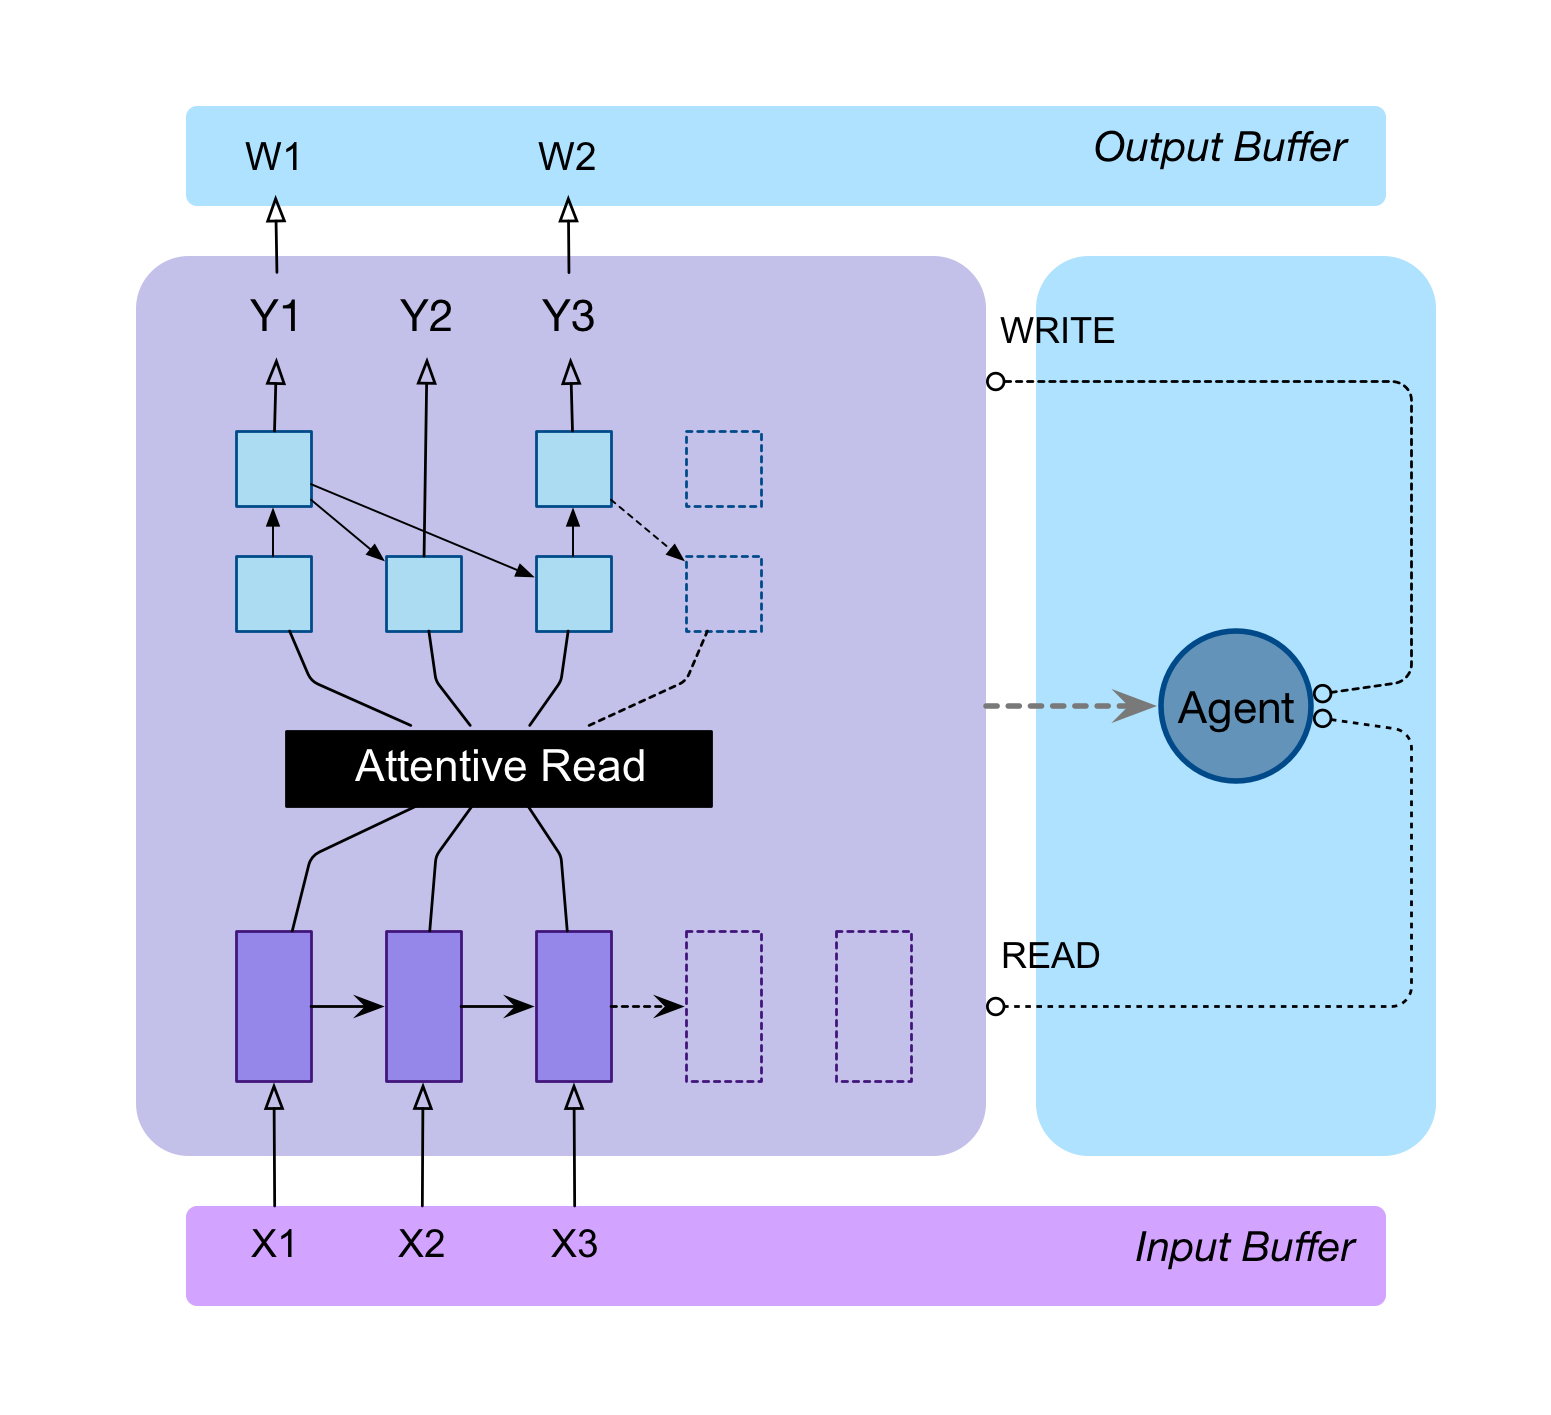
\includegraphics[scale=0.20]{./images/SNMT0}
\caption[Structure of a Simultaneous Neural Machine Translation.]{Structure of a Simultaneous Neural Machine Translation. At each time step the environment calculates $y_i$ and the agent decides whther to send to output buffer or wait for better translation.}
\label{fig:SNMT0}
\end{figure}

%In the first section of this chapter we will talk about a new approach to solve the task of translation in real-time, presented by Cho et al. We will look at a novel decoding algorithm, called \textit{Simultaneous greedy decoding} which serves as the starting point of  new family of algorithms to allow neural translation systems begin translating before receiving the full sentence. Then we will describe another method based on simultaneous greedy decoding in section \ref{sec:TA}, which shows us how we can train our systems to learn when to segment a sentence based on predefined quality and delay criteria.

\section{Neural Translation Environment} \label{sec:NTE}
The translation environment is very similar to attention-based Encoder-Decoder MT system which is described in section \ref{sub:attention} with some refinements. More precisely, the environment uses multi-layer LSTM networks where the Encoder receives the embedded representation of input sentences $X=\{x_1, \dots, x_{T_x}\}$ and converts them into context vectors $H=\{ h_1, \dots, h_{T_s} \}$ such that:
$$ h_n = f_{\textrm{ENC}}(x_n, h_{n-1}) $$
Since we do not have access to the whole sentence after $n$ READs ($n < T_x$), we will use $H^n$ which contains those context vectors that have been read so far (i.e. $H^n = \{ h_1, \dots, h_{n} \}$).\\
The Decoder is trained to generate target word, given the context vectors $H^n$, previous predicted word $w_{m-1}$ and previous decoder state $z_{m-1}$ after $n$ READs and $m$ WRITEs. for $t = n + m$ we will have:
\begin{align*}
    &c_{t} = a_{\textrm{ATT}}(z_{m-1}, H^n)\\
    &s_{t} = f_{\textrm{DEC}}(z_{m-1}, w_{m-1}, c_t)\\
    &p(y_t|w_{<{m}}, H^n) = g(w_{m-1}, z_m, c_t)
\end{align*}
Where $a$, $f$ and $g$ are nonlinear functions. The word with highest probability will be selected as output at each time step:
$$y_t = \arg \max_y p(y|w_{<m}, H^n)$$

One frequent point of confusion in the new translation model is that, in contrast to standard NMT model, we will have an output at each time $t$; However, the agent decides whether to ignore the current candidate ($y_t$) and wait for better predictions [READ], or accept the candidate ($w_m \leftarrow y_t$, $z_m \leftarrow s_t$) and select it as the next
translated word [WRITE].

\section{Various Types of Agent} \label{sec:Agent}
A separate agent is responsible for generating sequence of actions $A = \{ a_1, \dots, a_T \}$ where $a_i \in \{ \text{READ}, \text{WRITE} \}$, in order to maximize the translation quality and minimize delay. A non-trainable agent by Cho et al. \cite{cho:2016:Arxive} is described in \ref{sub:SNMT1}. Then in \ref{sub:SNMT2} and \ref{sub:SNMT3} we will explain how we can apply reinforcement learning techniques to create trainable agents.

\subsection{Greedy Decoding}\label{sub:SNMT1}
The non-trainable agent in \cite{cho:2016:Arxive}, controls the translation environment by heuristic modification of decoding process. The algorithm is depicted in Algo. \ref{alg:SGD}. For the rest of this report, \emph{SGD} would be referred as abbreviated form of "Simultaneous Greedy Decoding" algorithm.

%%%%%%%%%%%%%%%%%%%%%%%%%%%%%%%%%%%%%%%%%%%
\begin{algorithm}[H]
\caption{Simultaneous Greedy Decoding (SGD)}
\begin{algorithmic}[1] \label{alg:SGD}
\REQUIRE NMT system $\phi$, Policy $\pi_{\theta}$, $m_{\text{MAX}}$,\\
         input buffer $X$, output buffer $Y$, state buffer $S$.

\STATE \textbf{Init} $x_1 \Leftarrow X$, $h_1 \leftarrow f_{\text{ENC}}(x_1) $, $H^{1} \leftarrow \{h_1\}$,\\
    $z_0 \leftarrow f_{\text{INIT}}(H^1)$, $w_0 \leftarrow \langle s \rangle$, $m \leftarrow 0$, $n \leftarrow 1$

\WHILE{\text{True}}
\STATE $t \leftarrow m + n $
\STATE $c_{t} = a_{\textrm{ATT}}(z_{m-1}, H^n)$
\STATE $y_{t}, s_{t}, o_{t} \leftarrow \phi(z_{m-1}, w_{m-1}, c_{t})$
%=======
\IF{$\Lambda(t) = \text{READ}$ and $n < T_x$}
\STATE $x_{n+1} \leftarrow X$, $h_{n+1} \leftarrow \phi_{\text{ENC}}(h_n, x_{n+1})$
\STATE $H^{n+1} \leftarrow H^{n} \cup \{ h_{n + 1} \}$, $n \leftarrow n + 1$
\IF{$|Y| = 0$} \STATE $z_0 \leftarrow \phi_{\text{INIT}}(H^{n})$ \ENDIF

%-----------
\ELSIF{$\Lambda(t) = \text{WRITE}$ or $n \geq T_X$}
\STATE $z_{m} \leftarrow s_{t}$, $w_{m} \leftarrow y_{t}$
\STATE $Y \Leftarrow w_{m}$, $m \leftarrow m + 1$
\ENDIF
%-----------
\IF{$y_{t} = \langle /s \rangle$} \STATE break \ENDIF
%=======
\ENDWHILE
\end{algorithmic}
\end{algorithm}
%%%%%%%%%%%%%%%%%%%%%%%%%%%%%%%%%%%%%%%%%%%

The translation process is as follows. At each time step $t$, if the full source sentence is already received then the most likely word $y_t$ will be printed to the output; Otherwise, more source words will be passed through the network. The Agent compares the log probability of the most likely word at current time step with previous time step based on a predefined criterion $\Lambda$. If the agent decides to WRITE, then the environment commits the most likely target symbols $y_t$ given the current context set $C$ to the output; And if not, the environment will wait for more source words. Two waiting criteria $\Lambda$ has been studied in \cite{cho:2014:arxive}:

\begin{itemize}
    \item \textbf{Wait-If-Worse}
    The first scenario for the agent is to wait for more source words if the log probability of the most likely prediction decreases with more inputs. In other words, the criteria at time $t$ can be defined as:
    \begin{align*}
        &\Lambda(t) = 
        \begin{cases}
        \text{READ} & \text{if} \ \log p(y_t|w_{<{m}}, H^n) < \log p(y_t|w_{<{m}}, H^{n+1})\\
        \text{WRITE} & \text{otherwise}
        \end{cases}
    \end{align*}
    where $n$ and $m$ are the number of READs and WRITEs respectively at time $t$, and $y_t = \arg \max_y p(y|w_{<m}, H^{n}) $
    
    \item \textbf{Wait-If-Diff}
    The other scenario is to print the predicted word $y_t$ to the output, only if it won't change by reading more words from source sentence. Mathematically speaking, $\Lambda(t)$ can be described as:
    \begin{align*}
        &\Lambda(t) = 
        \begin{cases}
        \text{READ} & \text{if} \ y_t \neq y_{t+1}\\
        \text{WRITE} & \text{otherwise}
        \end{cases}
    \end{align*}
    where $y_{t+1} = \arg \max_y p(y|w_{<m}, H^{n+1}) $. This is different from previous criteria since decreasing log probability of a predicted word doesn't necessarily indicate that most likely word will be changed. 
\end{itemize}

By changing the policy, one can get various modes of translation. The standard NMT system can be achieved by setting policy to wait until the end of sentence which we call it \textbf{Wait-Until-End}. Also the fastest translator is the one which translates after receiving each word and we call it \textbf{Wait-One-Step}. 

\subsection{Trainable Agent with Q network}\label{sub:SNMT2}
The first trainable agent, introduced by Satija et al. \cite{harsh:2016:ICML} interacts with the environment (which in our case it is NMT system) using Reinforcement Learning algorithms. At each time step $t$, the agent receives an observation $o_t$ from the environment and chooses an action $a_t \in \{\text{READ}, \text{WRITE}\}$ which leads to a reward $r_t$ and transition into next observation $o_{t+1}$. The Q-learning techniques have been applied in order to estimate the value of executing an action from a given state, which are referred as Q-values. Then a deep neural network is employed to approximate the Q function, parametrized by weights denoted by $\theta$ \cite{mnih:2015:nature}. At time $t$, for a given observation $o_t$, the Q-values for all the available actions are predicted using this network and are denoted by $Q(a_t, o_t|\theta)$. The Q-values can be learned by making updates to the network to minimize the differentiable loss function:
$$ \mathcal{L}(a, o| \theta_i) \approx ( r + \gamma \max_{a'} Q(o', a'| \theta_i) - Q(o, a| \theta_i) )^2 $$
Where the updates are $Q_{i+1} = \theta_i + \alpha \nabla_\theta \mathcal{L}(\theta_i)$.
The other settings of their RL system is as follows:
\begin{itemize}
    \item \textbf{Observations}
    The observation of the agent represents its current view of the environment. It is represented as concatenation of the current Encoder's context vector $h_n$, The current Decoder's context vector $s_t$, and the last word predicted by environment $w_m$. Hence observation at time step $t$ can be written as $o_t = [\ h_n;\ s_t;\ w_m]$.
    \item \textbf{Reward}
    At each time $t$, the reward is computed as $r_t = r_t^Q \times r_t^D$ where $r_t^Q$ is the partial BLEU score for reference $Y^*$ which can be written as:
    \begin{align*}
        r_t^Q = 
        \begin{cases}
        \frac{1}{\beta}\text{BLEU}(Y^t, Y^*) &  t<T\\
        \text{BLEU}(Y, Y^*)                  &  t=T
        \end{cases}
    \end{align*}
    Where $Y$ is the output, $Y^t$ is the cumulative output at time $t$ and $\beta$ is the maximum sentence length permissible. $r_t^D$ is delay component of reward formula which can be calculated as:
    $$r_t^D = 1 - \frac{l-1}{\lambda}$$
    Where $\lambda$ is a fixed constant and $l$ represents the length of consecutive READ steps at time $t$.
\end{itemize}
We will now describe the translation process after pre-training of the NMT environment has been completed. Given a sentence, the Agent receives observation from the NMT system $o_t$ and generate the Q-values for the available actions using its own neural network. The agent then selects the action with the largest return and executes that. It gets a corresponding reward from the environment and also the next word from the source sequence, which sends it to the observation $o_t$. It keeps on executing in such manner until it receives terminal observation (the end of source sentence, represented by $\langle \text{eos} \rangle$ token) and after that the agent performs WRITE actions until the environment predict the $\langle \text{eos} \rangle$ token for the target sentence.

\subsection{Trainable Agent with Policy Gradient}\label{sub:SNMT3}
The most recent alternative for agent is presented by Gu et al. \cite{gu:2017:EACL}. Their model is similar to Satija's agent in a sense that they are using the same set of actions and the agent is trained with reinforcement learning techniques. However, as illustrated in Algo. \ref{alg:PG}, many aspects of the agent has been changed:
%%%%%%%%%%%%%%%%%%%%%%%%%%%%%%%%%%%%%%%%%%%
\begin{algorithm}[H]
\caption{Trainable agent with policy gradient}
\begin{algorithmic}[1] \label{alg:PG}
\REQUIRE NMT system $\phi$, Policy $\pi_{\theta}$, $m_{\text{MAX}}$,\\
         input buffer $X$, output buffer $Y$, state buffer $S$.

\STATE \textbf{Init} $x_1 \Leftarrow X$, $h_1 \leftarrow f_{\text{ENC}}(x_1) $, $H^{1} \leftarrow \{h_1\}$,\\
    $z_0 \leftarrow f_{\text{INIT}}(H^1)$, $w_0 \leftarrow \langle s \rangle$, $m \leftarrow 0$, $n \leftarrow 1$

\WHILE{$m < m_{\text{MAX}}$}
\STATE $t \leftarrow m + n $
\STATE $y_{t}, s_{t}, o_{t} \leftarrow \phi(z_{m-1}, w_{m-1}, c_{n})$
\STATE $a_t \sim \pi_{\theta}(a_t; a_{<t}, o_{<t})$
%=======
\IF{$a_t = \text{READ}$ and $x_n \neq \langle /s \rangle$ }
\STATE $x_{n+1} \leftarrow X$, $h_{n+1} \leftarrow \phi_{\text{ENC}}(h_n, x_{n+1})$
\STATE $H^{n+1} \leftarrow H^{n} \cup \{ h_{n + 1} \}$, $n \leftarrow n + 1$
\IF{$|Y| = 0$} \STATE $z_0 \leftarrow \phi_{\text{INIT}}(H^{n})$ \ENDIF

%-----------
\ELSIF{$a_t = \text{WRITE}$}
\STATE $z_{m} \leftarrow s_{t}$, $w_{m} \leftarrow y_{t}$
\STATE $Y \Leftarrow w_{m}$, $m \leftarrow m + 1$
\ENDIF

\IF{$y_{t} = \langle /s \rangle$} \STATE break \ENDIF
%=======
\ENDWHILE
\end{algorithmic}
\end{algorithm}
%%%%%%%%%%%%%%%%%%%%%%%%%%%%%%%%%%%%%%%%%%%

\begin{enumerate}
    \item \textbf{Observation} The current state in Cho's agent represented by concatenation of the current attention context vector $c_t$ , the current decoder state $s_t$ and the embedding vector of the candidate word $y_t$ as the continuous observation, $o(t) = [\ c_t ;\ s_t ;\ E (y_t )]$.
    \item \textbf{Reward}
    Although the model computes reward at the end of the sentence, it is calculated as cumulative sum of each time step. Hence, various evaluation metrics has been modified to be calculated at each time step.
    \begin{itemize}
        \item \textbf{BLEU Score}\\
        They decompose smoothed version of BLEU as described in section \ref{subsec:quality} and use the difference of partial BLEU scores as the reward, that is:
        \begin{align*}
            r_t^Q = 
            \begin{cases}
            \text{BLEU}(Y^t, Y^*) - \text{BLEU}(Y^{t-1}, Y^*) & t<T \\
            \text{BLEU}(Y, Y^*) & t=T
            \end{cases}
        \end{align*}
        Where $Y$ is the output, $Y^t$ is the cumulative output at $t$ and $Y^*$ is the reference.
        \item \textbf{Average Proportion}\\
        Following the definition in section \ref{subsec:delay}, Average proportion at each time step is calculated as:
        \begin{align*}
            &d_t = 
            \begin{cases}
            0       & t<T \\
            d(X, Y) & t=T
            \end{cases} \\[10pt]
            &d(X, Y) = \frac{1}{|X||Y|} \sum_t s(t)
        \end{align*}
        In other words, AP is calculated at the end of sentence and for all other time steps it would be zero.
        \item \textbf{Consecutive Wait}\\
        CW has been used as it is described and formulated in \ref{subsec:delay}.
    \end{itemize}
    The reward for delay $r_t^D$ is computed as combination of AP and CW, which has been devised as: 
    \begin{align}
        r_t^D = \alpha . [\text{sgn}(c_t - c^*)+1] + \beta . \lfloor d_t - d^* \rfloor
        \label{eq:reward}
    \end{align}
    Where $\alpha$, $\beta$, $d^*$, and $c^*$ are preset constants. Finally the total reward at each time step is achieved by setting $r_t = r_t^Q + r_t^D$.
\end{enumerate}

Instead of estimating state-value function, the new agent makes use of a softmax policy, which means parameters of policy $\pi_\theta$ is estimated by an RNN with a softmax function at final layer:
\begin{align*}
        &z_t = f_\theta (z_{t-1}, o_t) \\
        &\pi_\theta (a_t | a_{<t}, o_{\leq t}) \propto g_\theta(z_t)
\end{align*}
Where $z_t$ is the internal state of the agent. the RNN is then trained using policy gradient algorithm \cite{Williams:1992:ML}, which maximizes the following expected rewards:
$$J = \mathbb{E}_{\pi_\theta} \left[\sum_{t=1}^{T} r_t \right]$$
Whose gradient is:
$$\nabla_\theta J = \mathbb{E}_{\pi_\theta} \left[ \nabla_\theta \log 
    \pi_\theta \sum_{t=1}^{T} r_t \right]$$
Since we are computing this gradient at the end of sentence, it can be calculated as:
\begin{align*}
        \nabla_\theta J &= \mathbb{E}_{\pi_\theta} \left[ \sum_{t=1}^{T} \nabla_\theta \log \pi_\theta ( a_t | .) R_t \right] \\[10pt]
        R_t &= \sum_{k=t}^{T} \left[ r_k^Q + r_k^D \right]
\end{align*}
In practice, this gradient is estimated by sampling multiple action trajectories from the current policy $\pi_\theta$, collecting the corresponding rewards.\\

\section{Summary}
In this chapter, we have studied various proposed models for utilizing neural networks in simultaneous machine translation. All of the methods are similar in overall concept and are made up of a translation environment which output a word at each time step, and a separate agent in order to decide which output should be selected as actual output. But they are significantly different in structure of the agent. the detailed explanation of various agents is explained in section \ref{sec:Agent}. The results of each model will be discussed in the next chapter.

%++++++++++++++++++++++++++++++++++++++++++++++++++++++++++++++++++++++++++
\chapter{Results and Conclusion} \label{chap:results}
In this Chapter, we look at the results obtained by the methods discussed in Chapter \ref{chap:SNMT} and the comparison with each other is studied afterwards.
\section{Empirical Evaluation}
Since each method use their own parameters for environment and agent, we will start each of the following sub-sections by explaining the experimental settings for that model. Then the results are described and compared to other models.
\subsection{Greedy Decoding}
In order to study the proposed simultaneous greedy decoding algorithm, Cho et al. made use of corpora available from WMT 15\footnote{\url{http://www.statmt.org/wmt15/}} as training set and Newstest-2013 as Validation set and Test set. All the sentences were first tokenized and segmented into sub word units using byte pair encoding (BPE), which is a simple form of data compression in which the most common pair of consecutive bytes of data is replaced with a byte that does not occur within that data \cite{Gage:1994:Cusers}.
\\
The translation environment, consists of unidirectional recurrent network with 1028 Gated Recurrent Units for Encoder and Decoder. The soft-alignment function is a feedforward network with one hidden layer consisting of 1028 Tanh units. The model is trained with Adadelta \cite{zeiler:2012:arxive} until the average log-probability on the validation set does not improve. The quality evaluation for their pre-trained model can be found in Table \ref{table:sgdbleu}. The BLEU score for the pre-trained NMT model is lower than state-of-the-art NMT systems, Since the whole sentence is not accessible and the bidirectional RNN and many optimization techniques cannot be applied.

\begin{table}[h]
\centering
\begin{tabular}{ @{}r@{} | C || C C C}
\Tab{ \\ \Xhline{2\arrayrulewidth}
     \rotatebox{90}{~\parbox{0.64cm}{%
  En $\to$
}~} \\ \hline
 \rotatebox{90}{~\parbox{0.64cm}{%
  En $\gets$
}~}
}
&
\Tab{ \\ \Xhline{2\arrayrulewidth}
     Greedy Decoding \\[0.5ex] Baseline \\ \hline Greedy Decoding \\[0.5ex] Baseline}
&
\Tab{Cs \\ \Xhline{2\arrayrulewidth}
     15.2 \\[0.5ex] 13.84 \\ \hline 20.47 \\[0.5ex]  20.32}
&
\Tab{De \\ \Xhline{2\arrayrulewidth}
     19.5 \\[0.5ex] 21.75 \\ \hline 23.96 \\[0.5ex] 24}
&
\Tab{Ru \\ \Xhline{2\arrayrulewidth}
     17.77 \\[0.5ex] 19.54 \\ \hline 22.27 \\[0.5ex] 22.44}
\end{tabular}
\vspace{1cm}
\caption[BLEU score for the pre-trained NMT environment]{BLEU score for the pre-trained NMT environment compared to baseline NMT model \cite{Firat:2017:CSL}.}
\label{table:sgdbleu}
\end{table}
The performance of the framework in a real-time environment is illustrated in Figure \ref{fig:SGDres0}. Regardless of the waiting criterion, there is a clear trade-off between the translation quality and delay. Although it is more apparent with the Wait-If-Diff. Out of two waiting criteria, the Wait-If-Worse tends to achieve a better translation quality, while it has substantially higher delay in translation. The Wait-If-Diff criterion tends to cover wider spectra of the delay and the translation quality. On the other hand, with the same set of decoding parameters ($\delta$ and $s_0$), the Wait-If-Worse results in more delayed translation with less variance in translation quality.

\begin{figure}[h]
\centering
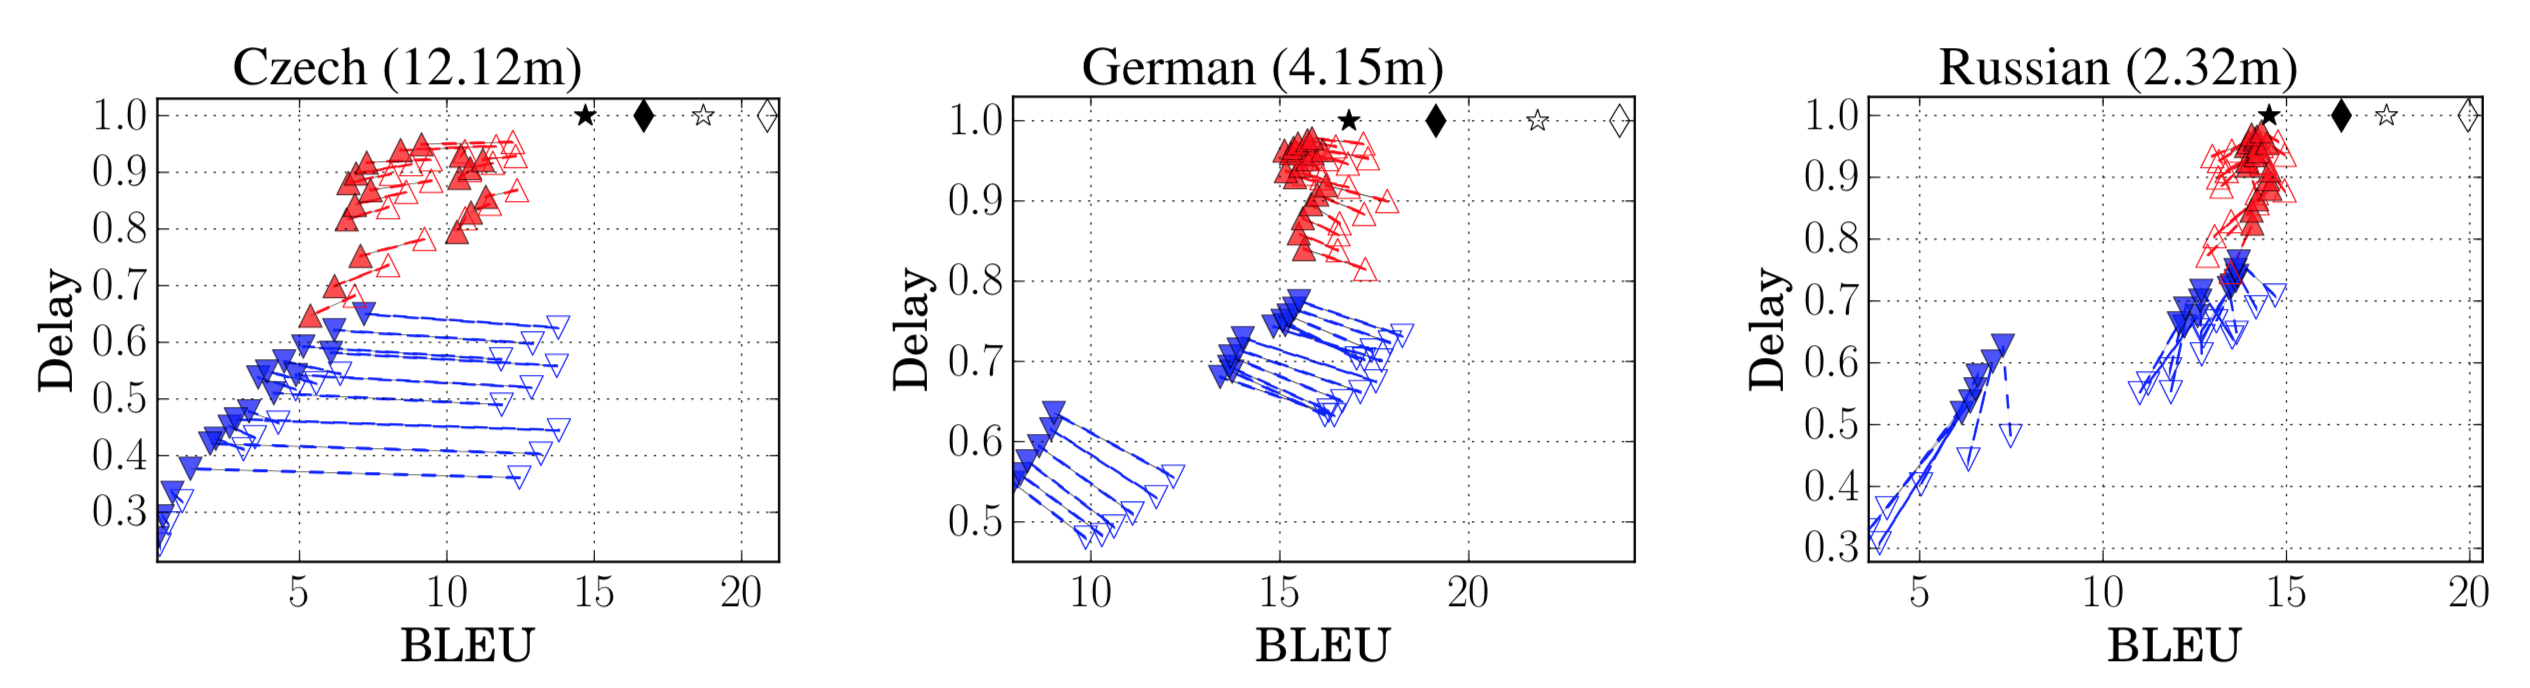
\includegraphics[scale=0.35]{./images/SGDres0}
\vspace{0.7cm}
\caption[Quality vs Delay for SGD in all language-pair direction]
{Quality(BLEU) vs Delay(AP) for all language pair direction.
\protect\marksymbol{$\blacktriangle$}{red}\quad : Wait-If-Worse (En $\rightarrow$).
\marksymbol{$\blacktriangledown$}{blue}\quad : Wait-If-Diff (En $\rightarrow$).
\marksymbol{$\triangle$}{red}\quad : Wait-If-Worse ($\rightarrow$ En).
\marksymbol{$\triangledown$}{blue}\quad : Wait-If-Diff ($\rightarrow$ En).
$\bigstar$ : consecutive greedy decoding (En $\rightarrow$).
$\blacklozenge$ : consecutive beam search (En $\rightarrow$).
\ding{73} : consecutive greedy decoding ($\rightarrow$ En).
$\lozenge$ : consecutive beam search ($\rightarrow$ En).
}
\label{fig:SGDres0}
\end{figure}
For the first time, \emph{simultaneous greedy decoding} algorithm explores the potential of neural machine translation frameworks in simultaneous translation and it's one of the first approaches that performs segmentation and translation jointly based solely on the translation quality; However, there are a number of points that needs to be further discussed:

\begin{enumerate}
    \item Their BLEU score is not good enough and even compared their standard NMT implementation, SGD algorithm remarkably reduced translation quality.
    \item The waiting criteria proposed in this paper are both manually designed and does not exploit rich information embedded in the hidden representation learned by the recurrent neural networks.
    \item The objective of the network is to improve translation quality and does not consider delay in producing the translation during training.
\end{enumerate}

\subsection{Trainable Agent with Q network}
Unfortunately, the model is not studied comprehensively, and performance evaluations are very restricted. they have used the bilingual parallel corpora from WMT' 14 translation task to train the NMT models, newstest-2014 as the development set, and newstest-2011 for test set. For the parameters of the reward function, they have used $\beta = 30$ and $\lambda = 10$.\\
They reported delay by the number of time-steps when agent is laying idle and is not producing any translation. Thus, delay is defined as the average number of READ actions the agent takes. sentences with maximum length 30 was selected from test set and statistics for them  plotted in Figure \ref{fig:qnetwork0}.\\

\begin{figure}[h]
\centering
\begin{tikzpicture}
\begin{axis}[
    xlabel={Delay - Avg number of waits},
    ylabel={Translation quality - BLEU score},
    xmin=-5, xmax=30,
    ymin=0.65, ymax=0.70,
    xtick={-5, 0, 5, 10, 15, 20, 25, 30},
    ytick={0.65, 0.66, 0.67, 0.68, 0.69, 70},
    legend pos=south east,
    scatter/classes={
	a={mark=triangle*,blue},
	b={mark=square*,blue},
	c={mark=*,blue},
	d={mark=triangle*,red},
	e={mark=square*,red},
	f={mark=*,red}}]
    
    \addplot[
    scatter, only marks,
    scatter src=explicit symbolic]
    coordinates  {
    		( 0  , 0.675) [c]
		( 14, 0.689) [b]
		( 23, 0.695) [a]
		( 0  , 0.658) [f]
		( 14, 0.680) [e]
		( 24, 0.684) [d]
    };
    \legend{FR WUE, FR Qnetwork, FR WOS, DE WUE, DE Qnetwork, FR WOS}
\end{axis}
\end{tikzpicture}
\vspace{0.7cm}
    \caption[Quality vs Delay for Q-network agent.]
{ Delay vs Translation Quality(BLEU) for EN-FR and EN-DE language pairs. The high BLEU score is due to the implementation they are using as defined in Section \ref{sub:SNMT2}. (WUE=Wait-Until-End, WOS=Wait-One-Step).}
\label{fig:qnetwork0}

\end{figure}

From Figure \ref{fig:qnetwork0} we can observe that the standard NMT system has much higher delay and the best translation score, whereas the worst policy which is Wait-One-Step) has no delay but has the worst BLEU score. This is expected behaviour as the standard NMT system has access to the entire input sequence and thus has the highest potential to produce the best translation but for Wait-One-Step the agent is forced to produce translation at each time-step. The Q-network has lesser delay than the NMT system but better translation quality than the Wait-One-Step policy. This shows that the agent is able to achieve better trade-off performance between quality and delay.

In contrast to previous approaches, The model proposed by Satija et al. makes use of reinforcement learning in order to create a separate agent for segmentation; However, their results cannot be compared to other methods, since they have defined their own metric for translation quality and delay. Besides, the model still reduce translation quality notably in comparison with Wait-Until-End, and do not demonstrate gains over traditional systems.  

\subsection{Trainable Agent with Policy Gradient}
Similar to Simultaneous Greedy Decoding, Gu et al. \cite{gu:2017:EACL} made use of the parallel corpora available from WMT' 15 for both pre-training the NMT environment and learning the policy. they have used newstest-2013 as the validation set to evaluate the proposed algorithm.\\
Similar to the settings in \cite{cho:2016:Arxive}, the NMT environment consists one GRU layer with 1028 units for both encoder and decoder. The agent is built using a recurrent policy with 512 GRUs and a softmax function to produce the action distribution. The agents are trained using policy gradient with Adam \cite{Kingma:2014:arxive} optimizer and a mini-batch size of 10. For each sentence pair in a batch, 5 trajectories are sampled.\\
In order to evaluate the effectiveness of their reinforcement learning algorithm with different reward functions, they vary the target delay $d^* \in \{\ 0.3,\ 0.5,\ 0.7\}$ and $c^* \in \{\ 2,\ 5,\ 8\}$ for Eq. \ref{eq:reward} separately, and trained agents with $\alpha$ and $\beta$ adjusted to values that provided stable learning for each language pair according to the validation set.

\begin{figure}[h]
\centering
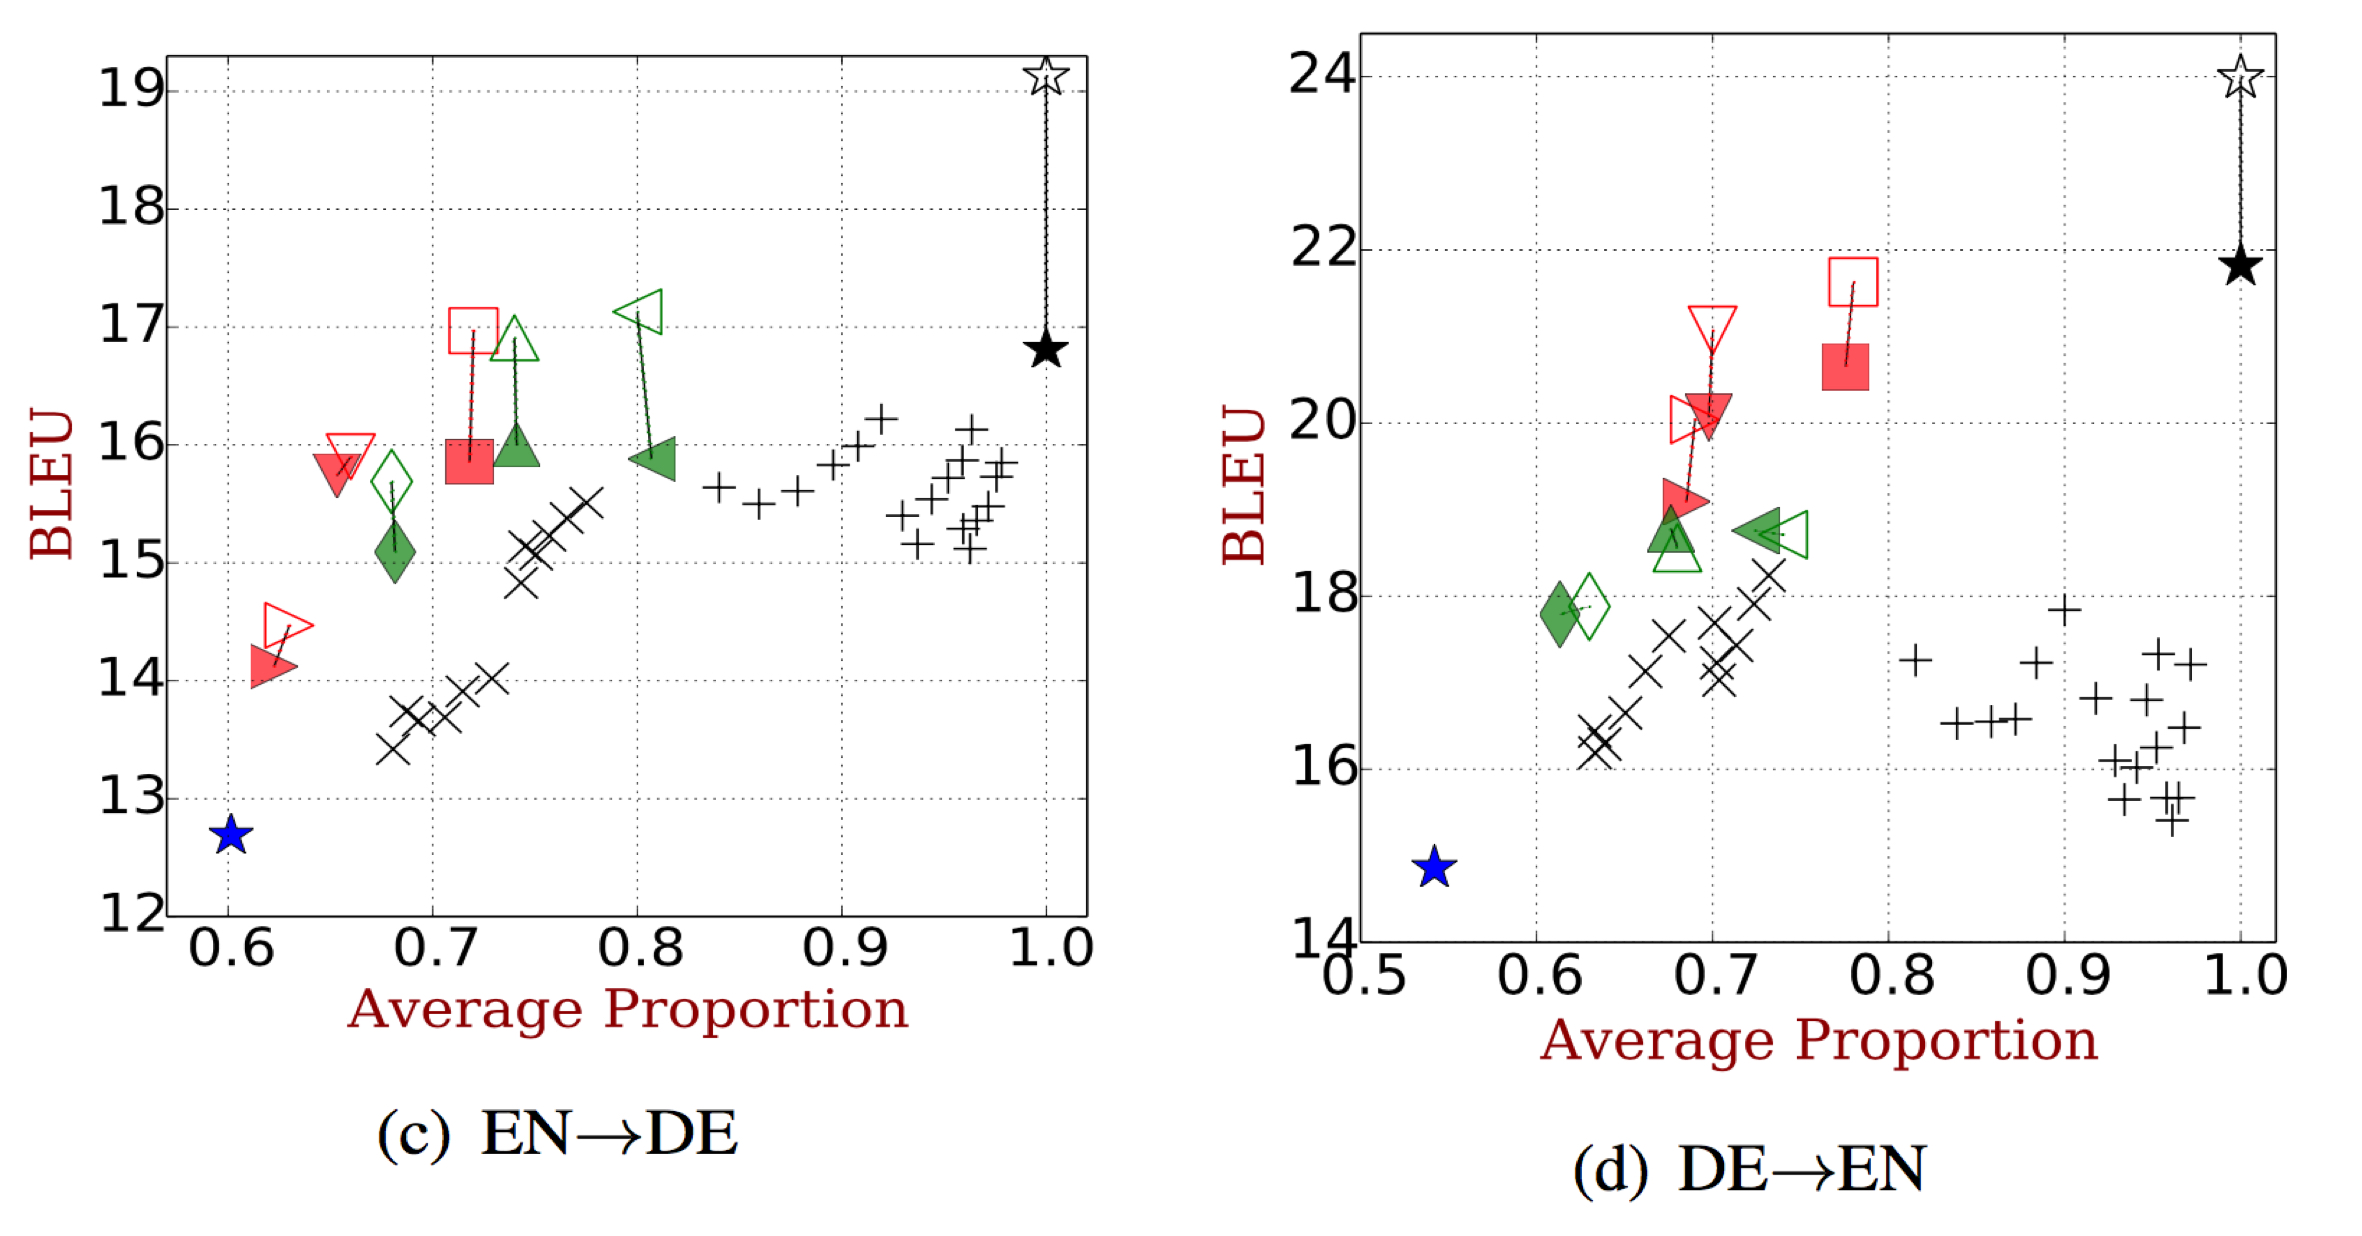
\includegraphics[scale=0.17]{./images/EN-DE}
\vspace{0.7cm}
\caption[Quality(BLEU) vs Delay(AP) for policy gradient agent.]
{Delay(AP) vs Quality(BLEU) for EN-DE language pair. The shown point-pairs are the results of simultaneous greedy decoding and beam-search (beam-size = 5) respectively with models trained for various delay targets:
\marksymbol{$\blacktriangleleft \quad \vartriangleleft $}{black!40!green}\qquad : CW=8,
\marksymbol{$\blacktriangle \quad \triangle $}{black!40!green}\qquad : CW=5,
\marksymbol{$\blacklozenge \quad \lozenge $}{black!40!green}\qquad : CW=2,
\marksymbol{$\blacktriangleright \quad \vartriangleright $}{red}\qquad : AP=0.3,
\marksymbol{$\blacktriangledown \quad \triangledown $}{red}\qquad : AP=5,
\marksymbol{$\blacksquare \quad \square $}{red}\qquad : AP=0.7,
\marksymbol{$\bigstar$}{blue}\quad : WOS,
$\bigstar$ \ding{73} : WUE,
$\times$ : WID, $+$ : WIW. 
}
\label{fig:PG0}
\end{figure}

As shown in Figure \ref{fig:PG0}, the trade-off between translation quality and delay has very similar behaviors across both language pairs and directions. The smaller delay (AP or CW) the learning algorithm is targeting, the lower quality (BLEU score) the output translation. It is also interesting to observe that, it is more difficult for "$\rightarrow$ EN" translation to achieve a lower AP target while maintaining good quality, compared to "EN $\leftarrow$". In addition, the models that are optimized on AP tend to perform better than those optimized on CW, especially in "$\rightarrow$ EN" translation. German sentences tend to be longer than English, hence require more consecutive waits before being able to emit the next English symbol.

\begin{table}
\centering
 \begin{tabular}{|c | c | c | c |} 
 \hline
  & Standard MT BLEU & SMT BLEU & SMT Delay \\ [0.5ex] 
 \hline\hline
 Statistical approach & 21.04 & 20.88 & 0.70 \\ 
 \hline
Simultaneous Greedy Decoding & 19.5 & 15.9 & 0.79 \\
 \hline
Agent with Policy Gradient & 19.5 & 17 & 0.8 \\
 \hline
\end{tabular}
\vspace{7mm}
\caption[The best statistical method VS neural approaches for EN $\rightarrow$ DE]{Comparing translation quality (BLEU) and delay (AP) of neural approaches with the best statistical method for EN $\rightarrow$ DE language pair.}
\label{tab:Final}
\end{table}

Comparing to Q-networks, the policy gradient algorithm seems to be a better fit for the agent, since it directly tries to find the optimal policy by training a neural network; However, it's still reducing translation quality a lot. It also cannot perform well on translating from SVO languages like EN to SOV languages like DE. 

Table \ref{tab:Final} summarizes the performance of various methods. As we can see, The agent with policy gradient method can achieve better translation quality with similar delay compared to the agent with simultaneous greedy decoding algorithm; However, Both neural approaches cannot beat statistical method since their underlying MT system is not able to perform well with a unidirectional RNN.

\section{Conclusion}
The new direction of research in Simultaneous MT systems is to develop a neural-network-based MT system that learns how to segment a sentence. Over the last few years, the translation quality of standard MT systems has greatly improved by introducing NMT systems \cite{Sutskever:2014:NIPS}; However, up to now, neural methods for simultaneous translation cannot beat statistical approaches. Besides most of the challenges from statistical approaches (e.g. prediction, evaluation , ...) remained unanswered in the modern architectures.\\
In this report, we examined neural approaches for simultaneous MT frameworks. We have studied a number of proposed evaluation metrics for both quality and delay and the standard NMT process is explained afterwards. Then we have discussed how the batch MT system can be modified in order to work in a real-time environment. A thorough review on the recent agent's structures which improved the performance of segmentation task was also provided. At the end, we examined results of various approaches and analyzed the effect of each agent.


%   BACK MATTER  %%%%%%%%%%%%%%%%%%%%%%%%%%%%%%%%%%%%%%%%%%%%%%%%%%%%%%%%%%%%%%
%
%   References and appendices. Appendices come after the bibliography and
%   should be in the order that they are referred to in the text.
%
%   If you include figures, etc. in an appendix, be sure to use
%
%       \caption[]{...}
%
%   to make sure they are not listed in the List of Figures.
%

\backmatter%
	\addtoToC{Bibliography}
	\bibliographystyle{plain}
	\bibliography{references}

%\begin{appendices} % optional
%	\chapter{Code}
%\end{appendices}
\end{document}
